\documentclass[11pt]{article}
\pdfinfoomitdate=1
\pdftrailerid{}
\pdfsuppressptexinfo=15
\usepackage[T1]{fontenc}
\usepackage[utf8]{inputenc}
\usepackage{lmodern,microtype}
\usepackage[a4paper,margin=28mm]{geometry}
\usepackage{amsmath,amssymb,amsthm,mathtools,booktabs,longtable,array}
\usepackage{tikz}
\usetikzlibrary{arrows.meta,positioning,calc}
\usepackage{xcolor}
\usepackage[colorlinks=true,linkcolor=blue!45!black,citecolor=blue!45!black,urlcolor=blue!45!black]{hyperref}
\usepackage{enumitem}
\setlist{topsep=5pt,itemsep=3pt}
\setcounter{tocdepth}{2}
\newtheorem{theorem}{Theorem}[section]
\newtheorem{lemma}[theorem]{Lemma}
\newtheorem{proposition}[theorem]{Proposition}
\newtheorem{corollary}[theorem]{Corollary}
\theoremstyle{definition}
\newtheorem{definition}[theorem]{Definition}
\newtheorem{remark}[theorem]{Remark}
\newcommand{\kk}{k}
\DeclareMathOperator{\Hom}{Hom}
\DeclareMathOperator{\Ext}{Ext}
\DeclareMathOperator{\End}{End}
\DeclareMathOperator{\rad}{rad}
\DeclareMathOperator{\soc}{soc}
\DeclareMathOperator{\coker}{coker}
\DeclareMathOperator{\im}{im}
\DeclareMathOperator{\id}{id}
\DeclareMathOperator{\Tor}{Tor}
\DeclareMathOperator{\Tr}{Tr}
\newcommand{\stHom}[3]{\underline{\Hom}_{#1}(#2,#3)}
\newcommand{\stEnd}[2]{\underline{\End}_{#1}(#2)}
\newcommand{\D}{\operatorname{D}}
\newcommand{\op}{\mathrm{op}}
\newcommand{\cone}{\operatorname{cone}}
\numberwithin{equation}{section}
\hypersetup{pdftitle={An explicit counterexample to the Auslander-Reiten conjecture},pdfauthor={OpenAI}}
\title{An explicit counterexample to the Auslander--Reiten conjecture}
\author{OpenAI}
\date{September 23, 2026}
\begin{document}
\maketitle
\begin{abstract}
We disprove the Auslander--Reiten conjecture for Artin algebras.
We construct a finite-dimensional algebra $\Lambda$ over
$k=\mathbb F_2(q,H_1,H_2)$ and a finite-dimensional nonprojective left module
$Z$ such that $\Ext^i_\Lambda(Z,Z)=\Ext^i_\Lambda(Z,\Lambda)=0$ for every
$i>0$. The module is Gorenstein-projective, so the same example also
disproves the Gorenstein-projective conjecture. Both counterexamples
persist after every extension of $k$.
\end{abstract}
\tableofcontents
\section{Introduction}

The Auslander--Reiten conjecture asks whether a finitely generated module
$M$ over an Artin algebra $R$ must be projective when
\begin{equation}\label{eq:arc}
 \Ext_R^i(M,M\oplus R)=0\qquad\text{for every }i>0.
\end{equation}
Here an Artin algebra is finite over a commutative Artinian central base
ring. In particular, every finite-dimensional algebra over a field is
an Artin algebra. The conjecture originates in the work of Maurice Auslander and
Idun Reiten on the generalized Nakayama conjecture
\cite{AuslanderReiten1975}; its module and generator formulations are
recalled in \cite[Introduction]{HunekeLeuschke2004}.

We give a counterexample. A module is called \emph{Gorenstein-projective}
if it is a cokernel in a doubly infinite exact complex of finite
projectives that remains exact after applying $\Hom_R(-,R)$.
The \emph{Gorenstein-projective conjecture} asks whether a finite
Gorenstein-projective module $M$ with $\Ext_R^i(M,M)=0$ for every
$i>0$ must be projective~\cite[p.~2]{LuoHuang2008}. The ambient algebra
is not assumed to be Gorenstein. Total acyclicity gives
$\Ext_R^i(M,R)=0$ for $i>0$, so this conjecture is precisely the
restriction of the Auslander--Reiten conjecture to Gorenstein-projective
modules.

\begin{theorem}\label{thm:main}
Let $\kk=\mathbb F_2(q,H_1,H_2)$, where $q,H_1,H_2$ are algebraically
independent. There exist a finite-dimensional $\kk$-algebra $\Lambda$
and a finite-dimensional nonprojective left $\Lambda$-module $Z$ such that
\[
 \Ext^i_\Lambda(Z,Z)=0=\Ext^i_\Lambda(Z,\Lambda)
 \qquad\text{for every integer }i\geq1.
\]
The module $Z$ is Gorenstein-projective. The semisimple quotient is
$\Lambda/\rad\Lambda\simeq\kk^8$, so the algebra is split with eight
isomorphism classes of simple modules; also $\rad(\Lambda)^4\ne0$.
These conclusions persist after every field extension of $\kk$.
\end{theorem}

Thus both conjectures fail for Artin algebras, including finite-dimensional
algebras over an algebraically closed field of characteristic two:
one can extend scalars to an algebraic closure of $\kk$. The parameters
play essential roles in the proof. The powers of $q$ give an infinite
resolution with uniform kernel formulas, and $H_1/H_2$ has infinite
multiplicative order. The algebraic closure in this assertion contains
these transcendental elements.

The final algebra is triangular and noncommutative. The companion article
\cite[Theorem~1.1 and Corollary~1.2]{OpenAITachikawa2026} constructs a
symmetric counterexample over the
same field by a different bimodule construction and a transfer requiring
control of negative complete self-extensions, and develops the
homological consequences of its associated endomorphism algebra.
The contribution here is
the explicit eight-simple Gorenstein-projective example and its persistence
under every field extension. Each paper contains its own complete proof.
The commutative restriction is not resolved by either construction; see
\cite[Appendix A]{ChristensenHolm2010} for its relationship with the
various Auslander and Tachikawa conditions.
The generator formulation also fails: $Z\oplus\Lambda$ is a
nonprojective generator with no positive self-extensions. Indeed Ext is
additive in both arguments, and all positive Ext groups with first
argument $\Lambda$ vanish.

\subsection{Earlier constructions and restricted results}

The positive cases developed along several lines. For the commutative
Noetherian formulation, Auslander, Ding and Solberg treated complete
local complete intersections by lifting across
regular sequences \cite[Proposition~1.9]{AuslanderDingSolberg1993}.
Huneke and Leuschke proved the conjecture for excellent commutative
Cohen--Macaulay normal domains containing the rational numbers, among
other classes \cite[Theorem~0.1]{HunekeLeuschke2004}.
Christensen and Holm established a general cohomological criterion:
every left-noetherian ring satisfying Auslander's condition satisfies
the conjecture \cite[Theorem~A]{ChristensenHolm2010}. That condition
requires, for each fixed finitely generated first module, a common bound
after which Ext vanishes for every finitely generated second module whose Ext groups
vanish eventually.

Algebras with radical cube zero form another important positive class.
Huneke, \c{S}ega and Vraciu treated commutative Artinian local rings
\cite[Theorem~4.1(1)]{HunekeSegaVraciu2004}. For split finite-dimensional
local algebras with radical cube zero, Ringel and Zhang proved the
stronger assertion that every nonprojective module with no positive
Ext to the algebra has a nonzero first self-extension
\cite[Theorem~1.5]{RingelZhang2022}.
Zhang and Zhou subsequently proved the conjecture for split
finite-dimensional algebras with radical cube zero
\cite[Theorem~1.1]{ZhangZhou2026}. Their result for Igusa--Todorov
Artin algebras includes all Artin algebras with radical cube zero
\cite[Theorem~3.2 and Corollary~4.4]{ZhangZhouIgusaTodorov2026}.
The algebra constructed here has nonzero fourth radical power, as
proved in Proposition~\ref{prop:radical}.

Schulz's construction of a nonprojective module without self-extensions
\cite{Schulz1994} is an important antecedent, but its particular
skew-field example lies outside the Artin-algebra setting above; see
\cite[Introduction]{DiverisPurin2012}. A separate distinction is between
all-degree and eventual vanishing: both summands in \eqref{eq:arc}
must vanish in every positive degree.

Schulz also exhibited two-dimensional modules over quantum exterior
algebras whose syzygies move through a parameter family and whose
self-extensions vanish eventually, while the first self-extension
remains nonzero \cite[Example~7]{Schulz1995}. The corresponding quantum
exterior algebra occurs as a corner of our starting algebra. We use
the same parameter-shifting mechanism for a resolution over a larger
algebra, then remove every positive self-extension by two independent twists.
For indecomposable weakly symmetric algebras over an algebraically closed
field with $J^3=0\ne J^2$, Erdmann characterizes those admitting
nonprojective modules with eventually vanishing self-extensions
\cite{Erdmann2017}; eventual vanishing alone does not give
\eqref{eq:arc}.
Xia proves the Auslander--Reiten conjecture for quantum complete
intersections \cite{Xia2026}, including the quantum exterior algebras
used in Schulz's parameter-shifting examples.

Vanishing in a finite range also differs from the hypothesis of
\eqref{eq:arc}. B\"ohmler and
Marczinzik \cite[Theorem 3.1 and the end of Section 3]{BoehmlerMarczinzik2026}
construct a characteristic-two commutative self-injective example with
vanishing first and second self-extensions, and nonzero third
self-extension.

Tachikawa's second conjecture is the self-injective case of
\eqref{eq:arc}. Enomoto proves that this conjecture for
the two-fold trivial extension of an Artin algebra implies the
Auslander--Reiten conjecture for that algebra
\cite[Theorem~3.1]{Enomoto2026}. His reduction produces a self-injective
algebra. The symmetric construction
in our companion and the structural assertions of Theorem~\ref{thm:main}
are separate contributions.

\subsection{How the construction removes self-extensions}

The proof has two parts. First we give a conversion principle: a
suitable stable map $v:X\to F\otimes_A X$ over a symmetric algebra
$A$ produces a module over
\[
 \Lambda=\begin{pmatrix}A&0\\F&A\end{pmatrix}.
\]
Its positive self-extensions are controlled by the difference between
the actions of a self-extension of $X$ on the two sides of $v$.
Total acyclicity separately gives the vanishing of Ext into $\Lambda$.
This principle is stated and proved before the example, so the
subsequent construction has an explicit target.

We then build the required $A,F,X,v$. Write $D$ for the $\kk$-linear dual.
A ten-dimensional algebra $C$
has a simple module $s$ whose Ext groups are especially sparse. Passing
to its symmetric trivial extension $T=C\ltimes DC$ produces
$\Ext_T^*(s,s)=\kk[\tau]$ with $|\tau|=3$. An explicit Hochschild
cocycle realizes $\tau$ and supplies a homotopy compatible with twists
of $T$. For $A=T\otimes T$ and $X=s\otimes s$, the nonnegative
self-extension algebra is $\kk[\tau_1,\tau_2]$.

Write $\mathcal C$ for the bimodule obtained from the two cones of
these classes. In the stable category, maps factoring through projective
modules are identified with zero, and the shift $[1]$ is inverse syzygy.
The stable maps from $X$ to
$(\mathcal C\otimes_A X)[a]$ form a line for $a=0$ and $a=3$ and
vanish in every other integer degree. This profile supplies a common
target for two differently twisted maps.

For a nonzero scalar $H$, let $h_H$ fix $C$ and scale $DC$ by $H$,
and let $U_H$ be $A$ with right action twisted by $h_H\otimes h_H$.
Its tensor functor fixes $X$ but multiplies its degree-$3m$
self-extensions by $H^{-m}$. Using the symmetrizing trace and the
cocycle's boundary identity, we construct maps $U_H\to\mathcal C[3]$
whose evaluations on $X$ are nonzero. After rescaling the maps for
$H_1$ and $H_2$, their evaluations are the same nonzero element of
that degree-three line.
Their finite fiber $F$ then has a single diagonal stable map
$v:X\to F\otimes_A X$ in degree zero, with both projections equal to
$\id_X$. In positive degrees, projection identifies the stable maps
from $X$ to $(F\otimes_A X)[a]$ with two copies of the self-extensions
of $X$. In degree $3m>0$, the comparison takes two independently chosen
self-extension classes $g,j$ to $F(g)v+v[3m]j$, where $F(g)$ denotes
tensoring with $F$. Under these projections its matrix is
\[
 \begin{pmatrix}H_1^{-m}&1\\H_2^{-m}&1\end{pmatrix}
 \otimes\id_{\kk[\tau_1,\tau_2]_{3m}}.
\]
This matrix is invertible for every $m>0$. In degree zero, the
comparison is surjective with a nonzero kernel. The conversion
principle therefore removes all positive self-extensions while keeping
a nonzero stable endomorphism, which proves nonprojectivity.

\begin{figure}[ht]
\centering
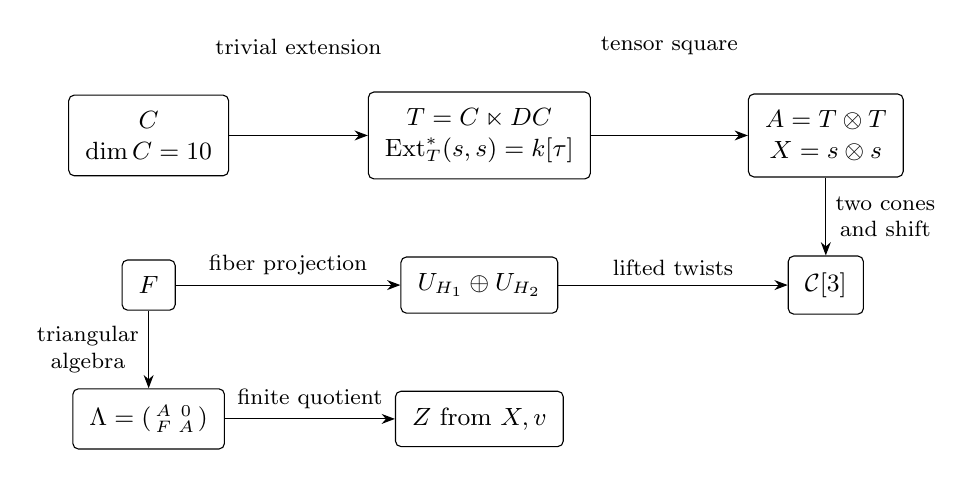
\begin{tikzpicture}[>=Stealth,every node/.style={font=\small},
 box/.style={draw,rounded corners=2pt,inner sep=6pt,align=center},
 lab/.style={font=\footnotesize,align=center}]
\node[box] (c) at (0,3.3) {$C$\\$\dim C=10$};
\node[box] (t) at (4.2,3.3) {$T=C\ltimes DC$\\$\Ext_T^*(s,s)=\kk[\tau]$};
\node[box] (a) at (8.6,3.3) {$A=T\otimes T$\\$X=s\otimes s$};
\node[box] (f) at (0,1.4) {$F$};
\node[box] (u) at (4.2,1.4) {$U_{H_1}\oplus U_{H_2}$};
\node[box] (cone) at (8.6,1.4) {$\mathcal C[3]$};
\node[box] (lam) at (0,-.3) {$\Lambda=\left(\begin{smallmatrix}A&0\\F&A\end{smallmatrix}\right)$};
\node[box] (z) at (4.2,-.3) {$Z$ from $X,v$};
\draw[->] (c)--node[above=9mm,lab]{trivial extension}(t);
\draw[->] (t)--node[above=9mm,lab]{tensor square}(a);
\draw[->] (a)--node[right,lab]{two cones\\and shift}(cone);
\draw[->] (f)--node[above,lab]{fiber projection}(u);
\draw[->] (u)--node[above,lab]{lifted twists}(cone);
\draw[->] (f)--node[left,lab]{triangular\\algebra}(lam);
\draw[->] (lam)--node[above,lab]{finite quotient}(z);
\end{tikzpicture}
\caption{The algebraic and homological stages of the construction.
The middle row begins the stable fiber triangle; the other arrows indicate
construction steps. The finite bimodule $F$ is the ordinary kernel in
\eqref{branch:finite-fiber} before $\Lambda$ is formed. Evaluating this
fiber on $X$ gives the diagonal stable map $v$; the final module is
the finite quotient \eqref{conv:finite-module}, using both $X$ and $v$.}\label{fig:construction}
\end{figure}

The main construction-specific ingredients are the explicit cocycle
with its twisted boundary identity, the lift through both cones, and
the resulting uniform comparison of the two twist actions. The
surrounding tools have a substantial history. Trivial extensions and
their Hochschild complexes are studied in
\cite{CibilsMarcosRedondoSolotar2003}; Hochschild evaluation as a
characteristic action is treated in \cite[Section~4.3]{Lowen2008}.
Bimodules attached to Hochschild classes and their iterated tensor products
occur in the support-variety constructions of Erdmann, Holloway,
Snashall, Solberg and Taillefer \cite[Section~2]{ErdmannEtAl2003}.
We use the natural symmetric stable duality of
\cite[Section 2]{Linckelmann2013} and the complete-resolution methods
of \cite{Veliche2006}. Gorenstein-projective modules over triangular
matrix rings are studied in \cite{EshraghiEtAl2014}. We supply the
particular comparison and finiteness arguments needed here.

For reference, the objects and their roles are summarized in
Table~\ref{tab:objects}. The finite cocycle table appears in
Appendix~\ref{app:cochain}; its identities are finite algebra
calculations. The resolution, duality, cone, and complete-resolution
arguments establish the assertions in all degrees.

Section~\ref{sec:stable} fixes the stable-category conventions, and
Section~\ref{conv:section} proves the conversion principle.
Sections~\ref{alg:section} and~\ref{res:section} give the starting
algebra and its self-extension calculation.
Section~\ref{cone:section} computes the two-cone profile;
Sections~\ref{sec:lift} and~\ref{branch:section} construct the lifts and
the finite fiber. Section~\ref{sec:consequences} proves the structural
and scalar-extension assertions.

\begin{table}[ht]
\centering\small
\begin{tabular}{@{}lll@{}}
\toprule
Object & Ambient algebra & Role or dimension\\
\midrule
$C$ & $\kk$ & ten-dimensional algebra\\
$T=C\ltimes DC$, $s$ & $\kk$, $T$ & symmetric algebra of dimension $20$; simple\\
$A=T\otimes T$, $X=s\otimes s$ & $\kk$, $A$ & symmetric algebra of dimension $400$; simple\\
$\mathcal C$ & stable bimodules over $A$ & two cones of degree-three classes\\
$U_{H_i}$ & $A$-bimodules & right twists of $A$\\
$F$ & $A$-bimodules & finite fiber, projective on both sides\\
$v:X\to F\otimes_A X$ & stable $A$-modules & both projections equal $\id_X$\\
$\Lambda$, $Z$ & $\kk$, $\Lambda$ & dimension $800+\dim_\kk F$; finite module\\
\bottomrule
\end{tabular}
\caption{Objects used in the proof. Shifts are homological.}
\label{tab:objects}
\end{table}

\section{Stable maps and complete resolutions}\label{sec:stable}

We first fix the language needed to pass from extension classes to an
ordinary finite module. All algebras and modules in the paper are
finite-dimensional over the indicated field. Modules are left modules
unless a side is specified. Write $DV=\Hom_\kk(V,\kk)$ and
$R^e=R\otimes_\kk R^{\op}$; an $R$-bimodule is a left $R^e$-module.
All tensor products without a subscript are over $\kk$.

Complexes have homological differentials $d_i:P_i\to P_{i-1}$ and shifts
$P[a]_i=P_{i-a}$. Thus a degree-$a$ cohomology class is represented by a
chain map $P\to Q[a]$. Throughout the construction
\[
 \kk=\mathbb F_2(q,H_1,H_2),
\]
where the three parameters are algebraically independent. Characteristic
two removes all differential, shift, and interchange signs.

For any finite algebra $R$, the space $\stHom{R}{M}{N}$ is the quotient
of $\Hom_R(M,N)$ by maps factoring through finite projective modules.
An algebra $R$ is \emph{symmetric} if it has a linear form $t:R\to\kk$
such that $t(ab)=t(ba)$ and $(a,b)\mapsto t(ab)$ is nondegenerate.
The resulting bimodule isomorphism $R\simeq DR$ shows that finite
projective $R$-modules are injective. Every finite module embeds in a
finite projective: dualize a finite projective surjection onto its dual.

For symmetric $R$, set $M[-1]=\Omega M$, the kernel of a projective
surjection onto $M$, and set $M[1]$ to be the cokernel of an embedding
of $M$ into a projective. These are well defined on stable maps and
inverse to each other there. Lifting through projective surjections and
extending into injectives give the maps on shifts; different choices
differ by projective factorizations. A short exact sequence induces a
stable triangle and long exact sequences of stable Hom groups in all
integer degrees. One concrete cone of $u:M\to N$ is the cokernel of
$(u,i):M\to N\oplus I$, where $i:M\hookrightarrow I$ is a projective
embedding. Its sequence is
\[
 M\xrightarrow{u}N\longrightarrow\cone(u)\longrightarrow M[1].
\]
The usual Hom and Ext sequences prove exactness in positive degrees.
At degree zero, maps through a projective lift through a surjection and
extend across an injection, giving exactness after quotienting by those
maps. Shifting gives every other degree. In particular,
\begin{equation}\label{eq:stable-ext}
 \stHom{R}{M}{N[a]}\simeq\Ext_R^a(M,N)\qquad(a>0),
\end{equation}
compatibly with composition and Yoneda products.

A \emph{complete resolution} of $M$ over a symmetric algebra is a doubly
infinite exact complex $P$ of finite projectives with
$M=\coker(d_1:P_1\to P_0)$. Splicing a projective resolution and an
injective coresolution constructs one. A complex of finite projectives
over an arbitrary finite algebra is \emph{totally acyclic} if both it and
$\Hom_R(P,R)$ are exact. Because every term is finitely generated, exactness into $R$
also gives exactness into every projective target, by direct sums and
summands. A module is \emph{Gorenstein-projective} if it
is such a cokernel in a totally acyclic complex. Complete resolutions
over symmetric algebras are totally acyclic. We will prove the precise
comparison with full Hom complexes in the next section; this also
applies over the final algebra, which need not be self-injective.

For an $A$-bimodule $F$, the notation $FM$ means $F\otimes_A M$.
If $F$ is projective as a left and as a right $A$-module, this is an
exact functor preserving finite projectives, hence induces a functor
on stable modules compatible with shifts. We always mean these two
separate projectivity conditions when describing a bimodule as
projective on both sides. They are weaker than projectivity over $A^e$.

\section{From two stable actions to a finite module}\label{conv:section}

The last step of the construction uses a finite bimodule $F$ and a stable
map $v:X\to F\otimes_A X$.  Two actions on maps out of $X$ will determine
all positive self-extensions of a module over a triangular algebra.  We
prove this conversion independently of the particular bimodule.  The
module itself is a finite quotient; complete resolutions are used to
compute its extensions.

\subsection{The conversion principle}

For a finite bimodule $F$ projective on both sides, tensoring with $F$
is exact and preserves projectives.  Over a symmetric algebra it
therefore induces an exact functor on the stable category and commutes
with shifts.  In the following statement we write $FX=F\otimes_A X$
and use these shift identifications when writing $F(g)$.

For the triangular algebra $\Lambda=\begin{pmatrix}A&0\\F&A\end{pmatrix}$,
we write a left module as a triple $(M,N,\eta)$: here $M,N$ are left
$A$-modules and $\eta:F\otimes_A M\to N$ is $A$-linear.  The action is
\[
 \begin{pmatrix}a&0\\f&b\end{pmatrix}(m,n)
       =(am,\eta(f\otimes m)+bn).
\]
A morphism $(\alpha,\beta)$ satisfies
$\beta\eta=\eta'(F\otimes\alpha)$.

\begin{proposition}[Triangular conversion]\label{conv:proposition}
Let $A$ be a finite-dimensional symmetric algebra over a field $\kk$
of characteristic two, let $F$ be a finite $A$-bimodule projective on
both sides, and let $X$ be a finite left $A$-module.  Suppose
$v\in\stHom{A}{X}{FX}$.  For each integer $a$, put
\[
 H^a=\stHom{A}{X}{X[a]},\qquad
 K^a=\stHom{A}{X}{(FX)[a]},
\]
and define
\begin{equation}\label{conv:delta}
 \delta^a:H^a\oplus H^a\longrightarrow K^a,
 \qquad (g,j)\longmapsto F(g)v+v[a]j.
\end{equation}
Assume that $\delta^0$ is surjective with nonzero kernel and that
$\delta^a$ is an isomorphism for every integer $a>0$.

Choose an actual map $v_0:X\to FX$ representing $v$ and an embedding
$i:X\to Q$ into a finite projective $A$-module.  Define
\begin{equation}\label{conv:finite-module}
 \Lambda=\begin{pmatrix}A&0\\F&A\end{pmatrix},\qquad
 Y=(FX\oplus Q)/\{(v_0(x),i(x)):x\in X\},\qquad
 Z=(X,Y,\iota),
\end{equation}
where $\iota:FX\to Y$ is induced by the first summand and specifies
the structure map of the left triangular module.  Then $Z$ is a finite
nonprojective Gorenstein-projective left $\Lambda$-module and
\[
 \Ext^a_\Lambda(Z,Z)=0=\Ext^a_\Lambda(Z,\Lambda)
 \qquad\text{for every integer }a>0.
\]
\end{proposition}

\subsection{Comparison of complete resolutions}

For homological complexes $P_\bullet,Q_\bullet$, use the full Hom complex
\begin{equation}\label{conv:full-hom}
 \Hom_R^a(P_\bullet,Q_\bullet)
   =\prod_{j\in\mathbb Z}\Hom_R(P_j,Q_{j-a}),
 \qquad
 (\partial f)_j=d^Q_{j-a}f_j+f_{j-1}d^P_j.
\end{equation}
This product convention is also used in \cite[Section 1.1.1]{Veliche2006}.
The product permits comparison maps with infinitely many nonzero
components.  Each component of the differential uses only two maps.
Its degree-$a$ cocycles are chain maps $P_\bullet\to Q_\bullet[a]$,
and its boundaries are nullhomotopic chain maps.  Throughout this section the
field has characteristic two, so the displayed signs apply to shifts
and cones as well.

\begin{lemma}[Complete-resolution comparison]\label{conv:comparison}
Let $R$ be a finite-dimensional algebra over a field of characteristic
two.  Let $P_\bullet$ be a totally acyclic complex of finite projective
left $R$-modules, and let $Q_\bullet$ be an exact complex of finite
projective left $R$-modules.  Put
\[
 C_j(P_\bullet)=\coker(d^P_{j+1}:P_{j+1}\to P_j),\qquad
 M=C_0(P_\bullet),\qquad N=C_0(Q_\bullet).
\]
There are natural, composition-compatible identifications
\[
 H^0\Hom_R^\bullet(P_\bullet,Q_\bullet)
       \simeq\stHom{R}{M}{N}.
\]
Applying this identification to shifted complexes gives, for every
integer $a$,
\begin{equation}\label{conv:shift-comparison}
 H^a\Hom_R^\bullet(P_\bullet,Q_\bullet)
 \simeq\stHom{R}{C_a(P_\bullet)}{N}
 \simeq\stHom{R}{M}{C_{-a}(Q_\bullet)}.
\end{equation}
For every integer $a>0$, these groups are naturally
$\Ext_R^a(M,N)$.
\end{lemma}

\begin{proof}
Exactness identifies $C_j(P_\bullet)$ with $\im d^P_j\subset P_{j-1}$.
We first record the extension property supplied by total acyclicity:
for every finite projective $T$, a map
$\phi:\im d^P_j\to T$ extends to $P_{j-1}$.  Indeed,
$\phi d^P_j:P_j\to T$ is a cocycle in $\Hom_R(P_\bullet,T)$.
Its exactness gives $\psi:P_{j-1}\to T$ with
$\psi d^P_j=\phi d^P_j$, which is the required extension.
This argument does not assume that projective $R$-modules are injective.

A chain map induces a map of cokernels.  Conversely, given $u:M\to N$,
first lift $u\epsilon_P$ to $f_0:P_0\to Q_0$, where $\epsilon_P$ and
$\epsilon_Q$ denote the quotient maps.  Projectivity and exactness give
$f_1,f_2,\ldots$ successively, with
$d^Q_jf_j=f_{j-1}d^P_j$.  To extend in the other direction,
$d^Q_0f_0$ kills $\im d^P_1=\ker d^P_0$.  It therefore induces a map
$\im d^P_0\to Q_{-1}$, which extends to $f_{-1}:P_{-1}\to Q_{-1}$ by
the preceding extension property.  The same argument gives
$f_{-2},f_{-3},\ldots$.  This constructs a full comparison map.

A nullhomotopy has components $h_j:P_j\to Q_{j+1}$ and satisfies
\[
 f_j=d^Q_{j+1}h_j+h_{j-1}d^P_j.
\]
On cokernels its first summand vanishes and its second factors through
$P_{-1}$.  Thus a nullhomotopic map induces a projective factorization.
For the converse, suppose the induced map factors as $M\to T\to N$
with $T$ finite projective.  Extend $M\to T$ to $P_{-1}$ by the extension
property, and lift $T\to N$ to $Q_0$.  Their composite is a homotopy
component $h_{-1}$ whose boundary induces exactly the given
factorization.  Subtract this boundary.  It remains to nullhomotope a
chain map $f'$ inducing zero on cokernels.

For this remaining map take $h_{-1}=0$.  Since $f'_0$ has image in
$\im d^Q_1$, projectivity gives $h_0:P_0\to Q_1$ with
$d^Q_1h_0=f'_0$.  Proceeding upwards, the residual
$f'_j+h_{j-1}d^P_j$ lands in $\ker d^Q_j=\im d^Q_{j+1}$ and hence
lifts to $h_j$.  Proceeding downwards from $j=-1$, the residual
$f'_j+d^Q_{j+1}h_j$ kills $\im d^P_{j+1}$ by the homotopy equation
already obtained at $j+1$.  It descends to $\im d^P_j$ and extends to
$h_{j-1}:P_{j-1}\to Q_j$ by the extension property.  Each recursion
assigns one component at a time and changes only adjacent equations.
Together they define a homotopy in the full product
\eqref{conv:full-hom}.  This proves the degree-zero identification.
Passing to cokernels respects composition, and the proved uniqueness
modulo homotopy gives its asserted compatibility.

Apply the degree-zero result to $P_\bullet[-a]$ or to
$Q_\bullet[a]$ to obtain \eqref{conv:shift-comparison}.  For $a>0$,
$C_a(P_\bullet)$ is the $a$th syzygy of $M$.  The projective-resolution
definition of $\Ext_R^a(M,N)$ quotients
$\Hom_R(C_a(P_\bullet),N)$ by maps extending to $P_{a-1}$.
These maps factor through a projective.  Conversely, every projective
factorization extends to $P_{a-1}$ by the extension property.  The two
quotients coincide, including when $a=1$.
\end{proof}

\subsection{Proof of the conversion principle}


\begin{proof}[Proof of Proposition~\ref{conv:proposition}]
We first check finiteness and introduce the two column functors.
Since $i$ is injective, the
map $\iota$ in \eqref{conv:finite-module} is injective and there is an
exact sequence
\begin{equation}\label{conv:finite-extension}
 0\longrightarrow FX\xrightarrow{\iota}Y
   \longrightarrow Q/i(X)\longrightarrow0.
\end{equation}
In particular all the modules in \eqref{conv:finite-module} are finite.
The algebra is finite as well, with
$\dim_\kk\Lambda=2\dim_\kk A+\dim_\kk F$.

The column functors below are standard; see \cite[Section 2]{EshraghiEtAl2014}.
Define
\[
 E(M)=(M,FM,\id),\qquad J(N)=(0,N,0).
\]
The functor $E$ is exact because $F$ is projective as a right
$A$-module; $J$ is exact directly.  Both preserve finite projectives:
$E(A)$ and $J(A)$ are the two projective columns of $\Lambda$, and
$\Lambda=E(A)\oplus J(A)$ as a left module.  The morphism condition
above gives
\begin{equation}\label{conv:four-homs}
\begin{aligned}
 \Hom_\Lambda(E(M),E(M'))&\simeq\Hom_A(M,M'),\\
 \Hom_\Lambda(J(N),J(N'))&\simeq\Hom_A(N,N'),\\
 \Hom_\Lambda(E(M),J(N))&=0,\\
 \Hom_\Lambda(J(N),E(M))&\simeq\Hom_A(N,FM).
\end{aligned}
\end{equation}
In the first line the lower component of a map is $F(\alpha)$.
The third line is a vanishing of ordinary module maps, so it holds
termwise for complexes in every shift.

Choose a complete resolution $P_\bullet$ of $X$ with
$P_{-1}=Q$ and $d_0=i\epsilon_P$.  This is possible by splicing a
projective resolution with a projective-injective coresolution, since
$A$ is symmetric.  Put
\[
 G_0=E(P_\bullet),\qquad G_1=J(P_\bullet).
\]
They are exact complexes of finite projective $\Lambda$-modules.
Moreover \eqref{conv:four-homs} gives
\begin{align*}
 \Hom_\Lambda(G_0,\Lambda)&\simeq\Hom_A(P_\bullet,A),\\
 \Hom_\Lambda(G_1,\Lambda)&\simeq
       \Hom_A(P_\bullet,F)\oplus\Hom_A(P_\bullet,A).
\end{align*}
These complexes are exact: the left $A$-modules $F$ and $A$ are
projective-injective.  Thus both $G_0$ and $G_1$ are totally acyclic.
Also $F\otimes_A P_\bullet$ is a complete resolution of $FX$.
Here right projectivity of $F$ gives exactness, left projectivity gives
projective terms, and self-injectivity of $A$ gives Hom exactness.

We can now compute all maps between the two induced complexes.
Lemma~\ref{conv:comparison} and \eqref{conv:four-homs} identify their
full Hom cohomology as
\begin{equation}\label{conv:column-cohomology}
\begin{aligned}
 H^a\End^\bullet_\Lambda(G_0)&\simeq H^a,
 &H^a\End^\bullet_\Lambda(G_1)&\simeq H^a,\\
 H^a\Hom^\bullet_\Lambda(G_1,G_0)&\simeq K^a,
 &\Hom^\bullet_\Lambda(G_0,G_1)&=0.
\end{aligned}
\end{equation}
Lift the actual map $v_0$ to a chain map $V:G_1\to G_0$ using the
comparison construction, and form
\[
 P_Z=\operatorname{Cone}(V),\qquad
 (P_Z)_j=(G_0)_j\oplus(G_1)_{j-1},\qquad
 d_j^{P_Z}=\begin{pmatrix}d^{G_0}&V_{j-1}\\0&d^{G_1}\end{pmatrix}.
\]
The degreewise split cone sequence shows that $P_Z$ is totally acyclic
with finite projective terms.

Its cokernel at degree zero is precisely the module $Z$ already
defined in \eqref{conv:finite-module}.  Its upper component is $X$.
For the lower component, first quotient $F\otimes_A P_0$ by the
image of $F\otimes_A d_1$, obtaining $FX$.  The remaining relations,
from $P_0$, are $(v_0(x),i(x))$: the lift $V_0$ induces $v_0$ on
cokernels and $d_0=i\epsilon_P$.  The resulting lower component is
therefore $Y$, with structure map $\iota$.  This supplies a complete
resolution of a concrete finite module.

It remains to compute its self-extensions.  Every graded endomorphism
of $P_Z$ has two diagonal blocks and one block from $G_1[1]$ to $G_0$;
the other direction vanishes by \eqref{conv:four-homs}.  Projection
to the diagonal gives a short exact sequence of cochain complexes
\begin{equation}\label{conv:end-sequence}
\begin{split}
0\longrightarrow\Hom^\bullet_\Lambda(G_1[1],G_0)
 \longrightarrow\End^\bullet_\Lambda(P_Z)
 \longrightarrow
 \End^\bullet_\Lambda(G_0)\oplus
 \End^\bullet_\Lambda(G_1[1])\longrightarrow0.
\end{split}
\end{equation}
This sequence is split in each graded degree, although the splitting
need not commute with the differentials.  Reindexing the full product
in \eqref{conv:full-hom} gives
\[
 H^a\Hom^\bullet_\Lambda(G_1[1],G_0)=K^{a-1}.
\]
The connecting map from diagonal degree $a$ to off-diagonal degree
$a+1$ is exactly \eqref{conv:delta}.  Indeed the differential of a
diagonal lift has cross term obtained by composing with $V$ on the
two sides.  The $E$-diagonal acts there by $F(g)$, and the $J$-diagonal
acts by precomposition with $j$, as specified in
\eqref{conv:four-homs}.  Compatibility of comparison with composition
identifies this cross term with $F(g)v+v[a]j$.

The long exact sequence of \eqref{conv:end-sequence} consequently
contains, for every integer $a$, the short exact sequence
\begin{equation}\label{conv:end-cohomology}
 0\longrightarrow\coker\delta^{a-1}
 \longrightarrow H^a\End^\bullet_\Lambda(P_Z)
 \longrightarrow\ker\delta^a\longrightarrow0.
\end{equation}
For $a=1$, surjectivity of $\delta^0$ and injectivity of $\delta^1$
make both outer terms zero.  For $a>1$, the two comparison maps are
isomorphisms.  Therefore the middle group vanishes for every $a>0$.
Lemma~\ref{conv:comparison} identifies it with
$\Ext^a_\Lambda(Z,Z)$.

At degree zero, \eqref{conv:end-cohomology} shows that
$H^0\End^\bullet_\Lambda(P_Z)$ surjects onto the nonzero kernel of
$\delta^0$.  By comparison this is a nonzero stable endomorphism
group of $Z$.  Its stable identity is consequently nonzero, since a
zero identity would annihilate every stable endomorphism.  Thus $Z$
is not projective.

Finally, total acyclicity gives exactness of
$\Hom_\Lambda(P_Z,\Lambda)$.  Its positive degrees compute the
ordinary groups $\Ext^a_\Lambda(Z,\Lambda)$ on the nonnegative
resolution tail, so these vanish for every $a>0$.  Exactness also
identifies $Z=\coker d_1^{P_Z}$ with the cycle
$\im d_0^{P_Z}=\ker d_{-1}^{P_Z}$ in this totally acyclic complex.
Hence $Z$ is Gorenstein-projective.
\end{proof}

Proposition~\ref{conv:proposition} reduces the construction to a finite
bimodule $F$ projective on both sides and a stable map $v$ with the stated two
action properties.  Surjectivity at degree zero is needed separately:
it is the term that removes a possible self-extension in degree one
in \eqref{conv:end-cohomology}.

\section{A symmetric algebra and a degree-three class}
\label{alg:section}

We begin with a symmetric algebra carrying a simple module and a
Hochschild class of degree three.  The class will have two uses: its
value on the simple will generate the positive self-extension algebra,
and an explicit boundary identity will allow us to lift maps through
the two cones used later.

\subsection{The ten-dimensional algebra and its trivial extension}

Let $C$ be the vector space with the following basis, arranged by
corners.  The notation $iCj$ specifies the left idempotent first.
\begin{equation}
\begin{array}{c|c@{\qquad}c|c}
 \text{corner}&\text{basis}&\text{corner}&\text{basis}\\ \hline
 eCe&e,x,y,z&eCf&u,v\\
 fCe&t,j&fCf&f,n
\end{array}
\label{alg:C-corners}
\end{equation}
The elements $e,f$ are orthogonal idempotents with sum $1$.  Besides
their actions specified by the corners, the complete list of nonzero
products is
\begin{equation}
\begin{gathered}
 xy=qz,\qquad yx=z,\qquad xu=yu=v,\qquad tx=j,\qquad ty=q^2j,\\
 ut=y+qx,\qquad vt=qz,\qquad uj=z,\qquad
 tu=(1+q)n,\qquad nt=qj,\qquad un=v.
\end{gathered}
\label{alg:C-products}
\end{equation}
All products not specified by these rules are zero.

\begin{lemma}\label{alg:C}
The rules \eqref{alg:C-corners}--\eqref{alg:C-products} define an
associative unital algebra of dimension ten.  Its radical is the span
of the eight non-idempotent basis vectors, and
\[
 (\rad C)^5=0,\qquad utut=q(1+q)z\ne0.
\]
\end{lemma}

\begin{proof}
Give $u,t$ degree one, $x,y,n$ degree two, $v,j$ degree three, and $z$
degree four; the idempotents have degree zero.  Every listed product
is homogeneous.  Associativity involving an idempotent follows from
the corners.  For three non-idempotent basis vectors, incompatible
corners or total degree greater than four force both bracketings to
vanish.  The complete remaining list is recorded below; direct
substitution gives the same value under either bracketing.
\[
\begin{array}{c|ccccccccccc}
 abc&utu&tut&xut&yut&ntu&unt&txu&tyu&utx&uty&tun\\ \hline
 (ab)c=a(bc)&(1+q)v&q(1+q)j&qz&qz&0&qz&0&0&z&q^2z&0
\end{array}
\]
This proves associativity by trilinearity.  The positive-degree span
$N$ is a nilpotent ideal with $N^5=0$ and $C/N\cong\kk\times\kk$;
therefore $N=\rad C$.  Finally, $(ut)u=(1+q)v$ and $vt=qz$ give the
asserted nonzero fourth radical product.
\end{proof}

\begin{remark}\label{alg:antecedent}
The corner $eCe$ is the quantum exterior algebra
$\kk\langle x,y\rangle/(x^2,y^2,xy-qyx)$, with $z=yx$.
The right module $fCe$ has basis $t,j$ and actions
$tx=j$, $ty=q^2j$, $jx=jy=0$. More precisely, put $R=eCe$.
The map
\[
 t\longmapsto x+q^{-1}y,\qquad j\longmapsto q^{-1}z
\]
identifies $fCe$ with the right ideal $(x+q^{-1}y)R$.
In the notation of Schulz \cite[Example~7]{Schulz1995}, the parameter
is $q^{-1}$ and this ideal is the first syzygy of $(x+y)R$.
Here its interactions with the other corners are fixed by the complete
multiplication table above.
\end{remark}

Put $L=DC$ and equip it with the dual bimodule actions
\begin{equation}
 (a\phi)(c)=\phi(ca),\qquad (\phi a)(c)=\phi(ac)
 \quad(a,c\in C,\ \phi\in L).
\label{alg:dual-actions}
\end{equation}
Trivial extensions and their cohomology are studied in \cite{CibilsMarcosRedondoSolotar2003}. Here the trivial extension is
\begin{equation}
 T=C\ltimes L,
 \qquad (a,\phi)(b,\psi)=(ab,a\psi+\phi b).
\label{alg:T-definition}
\end{equation}
For every lower-case basis letter $a$ of $C$, its upper-case letter
$a^*$ denotes the dual basis vector in $L$; for example, $j^*=J$ and
$f^*=F$.  We also set $(a^*)^*=a$.  Thus a capital letter $J$ is a
basis vector, whereas the radical below is denoted by $\mathfrak r$.

\begin{lemma}\label{alg:T}
The algebra $T$ is symmetric of dimension twenty.  A symmetrizing
trace is
\[
 \lambda(a,\phi)=\phi(1),
\]
and the trace-dual of each basis letter is its starred letter.  Its
radical $\mathfrak r$ is the span of all basis letters except $e,f$;
it satisfies $\mathfrak r^6=0$ and $T/\mathfrak r\cong\kk\times\kk$.
\end{lemma}

\begin{proof}
The dual actions satisfy the bimodule identities by associativity of
$C$, so \eqref{alg:T-definition} is associative.  Moreover,
\[
 \lambda\bigl((a,\phi)(b,\psi)\bigr)=\psi(a)+\phi(b),
\]
which is symmetric and nondegenerate.  In particular,
$\lambda(ab^*)=\delta_{a,b}$ for lower-case basis letters $a,b$.
The dual of the corner $iCj$ lies in $jLi$.

Extend the grading of $C$ by
$\deg(a^*)=5-\deg(a)$.  Formula \eqref{alg:dual-actions} shows that
every product in $T$ is homogeneous.  All basis vectors except $e,f$
have positive degree, and no degree exceeds five.  Their span is
therefore a nilpotent ideal whose quotient is $\kk\times\kk$;
this proves the radical assertions.
\end{proof}

Let $s$ be the one-dimensional left $T$-module on which $f$ acts as
$1$ and every other basis letter acts as zero.  It is inflated from
the corresponding $C$-simple.  Write $s^{\mathrm r}$ for the right
simple defined by the same character.

\subsection{The bar class and the finite identities}

Set $I=\kk e\oplus\kk f$.  The normalized relative bar resolution of
$T$ has terms
\begin{equation}
 P_n=T\otimes_I\mathfrak r^{\otimes_I n}\otimes_I T
 \quad(n\ge0),\qquad P_n=0\quad(n<0).
\label{alg:bar}
\end{equation}
We write $a_0[a_1|\cdots|a_n]a_{n+1}$ for an elementary tensor.  The
differential multiplies each adjacent pair of factors and sums the
results; the augmentation $P_0\to T$ is multiplication.  All signs
are $+$ because the characteristic is two.  Splitting by idempotents
expresses each term as a finite sum of projective bimodules
$Ti\otimes jT$ with $i,j\in\{e,f\}$.  Exactness follows from a contraction:
replace the first coefficient $a_0$ by its projection to
$\mathfrak r$, insert that projection as a new first bar, and put
$1$ in the first coefficient.  In augmented degree send $a$ to
$1[]a$.  Writing $\sigma$ for this contraction, the identity
$d\sigma+\sigma d=\id$ follows by canceling successive
multiplications; the $I$-component of $a_0$ is balanced over $I$.
This contraction is right $T$-linear, so $P\otimes_T s$ is a
projective resolution of $s$ as well.

Give a lower-case letter weight zero and an upper-case letter weight
one.  This weight records the effect of scaling the square-zero ideal
$L=DC$; it is distinct from the positive grading in
Lemma~\ref{alg:T}.  The complete table in Appendix~\ref{app:cochain}
defines an $I$-bimodule map
\[
 p:\mathfrak r\otimes_I\mathfrak r\otimes_I\mathfrak r\longrightarrow T.
\]
Every unlisted value is zero.  The following records exactly the
properties of this finite table that the proof needs.

\begin{lemma}\label{coc:data}
The cochain $p$ has weight $-1$ and is a Hochschild cocycle.  Its
associated class evaluated on $s$ is nonzero in $\Ext_T^3(s,s)$.

For any $H\in\kk^\times$, let $h=h_H$ be the automorphism of $T$
fixing $C$ and multiplying $L$ by $H$.  On the radical basis define
\[
 z_H(a)=
 \begin{cases}
 Hqa,&a\in\{u,v,t,E,X,Y,Z,U,V\},\\
 0,&\text{otherwise},
 \end{cases}
\]
and extend linearly.  For all $a,b\in\mathfrak r$ one has
\begin{equation}
 \sum_{w\in\mathcal B_{\mathfrak r}}
      p(a,b,h(w))w^*
  =a z_H(b)+z_H(ab)+z_H(a)h^{-1}(b),
\label{coc:boundary}
\end{equation}
where $\mathcal B_{\mathfrak r}$ is the radical basis.
\end{lemma}

\begin{proof}
The endpoint, weight, cocycle and boundary identities are verified
from the complete finite data in Appendix~\ref{app:cochain}.
We prove the nonzero evaluation explicitly.  In the bar complex
$s^{\mathrm r}\otimes_T P\otimes_T s$, consider
\begin{equation}
 \zeta=q^2[t|x|J]+[t|y|J].
\label{coc:cycle}
\end{equation}
Both words have endpoint $f$ on each side.  All outer radical
actions vanish on the endpoint simples.  The multiplication rules,
including the dual actions, give
\[
 tx=j,\qquad ty=q^2j,\qquad xJ=T,\qquad yJ=q^2T.
\]
Consequently
\[
 d\zeta=q^2([j|J]+[t|T])+q^2[j|J]+q^2[t|T]=0.
\]
The table gives $p(t,x,J)=0$ and $p(t,y,J)=q^3f$, so its evaluation on
$\zeta$ is $q^3\ne0$.  Every $T$-linear map from $P\otimes_T s$ to
$s$ factors through the left simple quotient and hence pairs with
this two-sided-simple bar complex.  A coboundary pairs to zero with
its cycles.  Thus the evaluated class is nonzero.
\end{proof}

The evaluation of a Hochschild class on modules is the characteristic action; see \cite[Section 4.3]{Lowen2008}. We use the same letter $p$ for its comparison map $P\to P[3]$:
for $n\ge3$ apply the cochain to the last three bars and multiply its
output into the right coefficient,
\begin{equation}
 a_0[a_1|\cdots|a_n]a_{n+1}\longmapsto
 a_0[a_1|\cdots|a_{n-3}]
 p(a_{n-2},a_{n-1},a_n)a_{n+1};
\label{coc:comparison}
\end{equation}
the map is zero for $n<3$.  This is a chain map: strict-prefix
multiplications cancel, and the remaining equation on the last
four bars is precisely the Hochschild cocycle equation.  At the
bottom index the target differential is zero.  Composing its
evaluation on $s$ with the augmentation represents the class in
Lemma~\ref{coc:data}.

We have now obtained the finite algebra and the specific degree-three
class.  The next step is to compute all self-extension degrees of
$s$, so that this nonzero class can be identified as a polynomial
generator.

\section{A simple module with polynomial self-extensions}
\label{res:section}

The cocycle constructed above will control the two cones in our example.
We now determine all self-extensions of the simple on which it acts.
The key step is a calculation over the smaller algebra $C$: its simple $s$
has no positive self-extensions, but $\Ext_C^2(s,C)$ is a simple module.
Passing to the trivial extension $T=C\ltimes DC$ turns this exceptional
class into a polynomial generator of degree three.

\subsection{The resolution over \texorpdfstring{$C$}{C}}

Let $s^{\mathrm r}$ denote the one-dimensional right $f$-simple.
For every integer $i\geq0$, set
\[
 \ell_i=x+q^i y.
\]
The transcendence of $q$ implies $q\ne0$ and $1+q^m\ne0$ for every
positive integer $m$. We will use these conditions for arbitrarily large
indices.

\begin{lemma}\label{res:base}
A projective resolution $R\to s$ over $C$ has terms
\[
 R_0=Cf,\qquad R_i=Ce\quad(i\geq1),
\]
and differentials given by right multiplication:
\[
 \cdots\longrightarrow Ce
 \xrightarrow{\,\cdot\ell_1\,}Ce
 \xrightarrow{\,\cdot\ell_0\,}Ce
 \xrightarrow{\,\cdot u\,}Cf\longrightarrow s\longrightarrow0.
\]
More precisely, $d_{i+2}$ is right multiplication by $\ell_i$ for every
$i\geq0$. For every integer $i\geq0$,
\[
 \Ext_C^i(s,s)=
 \begin{cases}\kk&i=0,\\0&i>0,\end{cases}
 \qquad
 \Ext_C^i(s,C)=
 \begin{cases}s^{\mathrm r}&i=2,\\0&i\ne2.\end{cases}
\]
The second identification is an identification of right $C$-modules.
\end{lemma}

\begin{proof}
The left ideals $Ce$ and $Cf$ have respective bases
\[
 (e,x,y,z,t,j),\qquad(f,u,v,n).
\]
The multiplication table gives the following formulas, valid for every
$i\geq0$:
\[
\begin{array}{c|cccccc}
 a&e&x&y&z&t&j\\ \hline
 au&u&v&v&0&(1+q)n&0\\
 a\ell_i&\ell_i&q^{i+1}z&z&0&(1+q^{i+2})j&0.
\end{array}
\]
Consequently, right multiplication by $u$ has image
$\langle u,v,n\rangle=\rad(Cf)$ and kernel
$\langle\ell_0,z,j\rangle$. Right multiplication by $\ell_i$ has image
$\langle\ell_i,z,j\rangle$ and kernel
$\langle\ell_{i+1},z,j\rangle$. In the latter calculation, a kernel vector
has zero $e$- and $t$-coefficients, while its $x,y$ coefficients satisfy
$a_y=q^{i+1}a_x$. These identities prove exactness at every index.
Since $\Hom_C(Ce,s)=es=0$ and $\Hom_C(Cf,s)=fs=\kk$, they also give the
asserted self-extension groups over $C$.

To compute $\Ext_C^*(s,C)$, identify
$\Hom_C(Ce,C)=eC$ and $\Hom_C(Cf,C)=fC$ by evaluation at the idempotent.
Precomposition with right multiplication becomes left multiplication.
Thus the Hom complex is
\[
 fC\xrightarrow{\,u\cdot\,}eC
 \xrightarrow{\,\ell_0\cdot\,}eC
 \xrightarrow{\,\ell_1\cdot\,}eC\longrightarrow\cdots.
\]
Left multiplication by $u$ sends the basis $(f,t,j,n)$ of $fC$ to
$(u,y+qx,z,v)$. These four vectors are independent. On the basis
$(e,x,y,z,u,v)$ of $eC$, left multiplication by $\ell_i$ is
\[
\begin{array}{c|cccccc}
 a&e&x&y&z&u&v\\ \hline
 \ell_i a&\ell_i&q^i z&qz&0&(1+q^i)v&0.
\end{array}
\]
The index $i=0$ is exceptional:
\[
 \ker(\ell_0\cdot)=\langle qx+y,z,u,v\rangle=\im(u\cdot),
 \qquad
 \im(\ell_0\cdot)=\langle\ell_0,z\rangle.
\]
For every $i\geq1$, the coefficient $1+q^i$ is nonzero, and
\[
 \ker(\ell_i\cdot)=\langle\ell_{i-1},z,v\rangle,
 \qquad
 \im(\ell_i\cdot)=\langle\ell_i,z,v\rangle.
\]
The cohomology in degrees zero and one therefore vanishes. In degree two
it is the line represented by $v$; in every higher degree the displayed
kernel equals the preceding image. Finally, $vf=v$, $ve=0$, and the only
possibly nonzero right radical product is $vt=qz$, which is a boundary.
The surviving line is precisely $s^{\mathrm r}$.
\end{proof}

\subsection{The trivial-extension triangle and its product}

Write $L=DC$. The duality calculation in Lemma~\ref{res:base} determines
$L\otimes_C^{\mathbf L}s$. The extension $0\to L\to T\to C\to0$
then provides a connecting morphism over $T$. We identify its products
explicitly so that the calculation controls every positive degree.

\begin{lemma}\label{res:polynomial}
For the algebra $T=C\ltimes DC$ and its left $f$-simple $s$,
\[
 \Ext_T^*(s,s)=\kk[\tau],\qquad |\tau|=3,
\]
as a graded algebra, where $\tau=p(s)$ is the evaluation of the cocycle
from Lemma~\ref{coc:data}.
\end{lemma}

\begin{proof}
For a finite projective left $C$-module $V$, evaluation gives a natural
isomorphism of left $C$-modules
\[
 DC\otimes_C V\longrightarrow D\Hom_C(V,C),\qquad
 \lambda\otimes v\longmapsto
 \bigl(\varphi\longmapsto\lambda(\varphi(v))\bigr).
\]
Apply this isomorphism termwise to the resolution $R$ of
Lemma~\ref{res:base}. Exactness of vector-space duality shows that
$L\otimes_C R$ has homology only in degree two, where it is
$D(s^{\mathrm r})=s$. Moreover, $L$ acts by zero on the entire complex,
since $L^2=0$. Good truncations therefore give a $T$-linear derived
identification
\[
 L\otimes_C R\simeq s[2].
\]

Regard $0\to L\to T\to C\to0$ as a sequence of $(T,C)$-bimodules.
Tensoring it termwise with $R$ gives a short exact sequence of complexes
of left $T$-modules,
\[
 0\longrightarrow L\otimes_C R
 \longrightarrow T\otimes_C R
 \longrightarrow R\longrightarrow0,
\]
where the last complex is inflated along $T\to C$. Exactness uses
projectivity of each left $C$-module $R_i$; it does not require flatness
of $L$ or $T$ as right $C$-modules. Put
$\mathcal I=T\otimes_C R$. We obtain the derived triangle
\begin{equation}\label{res:triangle}
 s[2]\longrightarrow\mathcal I\longrightarrow s
 \xrightarrow{\,\delta\,}s[3].
\end{equation}
The middle complex has homology $s$ in degrees zero and two and no other
homology. Its terms are finite dimensional, so good truncation makes
it an object of the bounded derived category of finite $T$-modules.

Each term of $\mathcal I$ is a finite projective $T$-module. Because the
complex is bounded below homologically, it computes derived maps out of
it: a map from it to an acyclic complex is nullhomotopic by successive
projective lifts starting in its bottom degree. Termwise induction and
restriction adjunction thus gives, for every integer $i$,
\[
 B^i:=\Hom_{D^b(T\text{-mod})}(\mathcal I,s[i])
 =H^i\Hom_C(R,s)
 =\begin{cases}\kk&i=0,\\0&i\ne0.\end{cases}
\]

Set $E^i=\Hom_{D^b(T\text{-mod})}(s,s[i])$. These are ordinary Ext
groups for $i\geq0$ and vanish for $i<0$. Applying
$\Hom(-,s[i])$ to \eqref{res:triangle} gives the exact segment
\begin{equation}\label{res:recurrence}
 B^{i-1}\longrightarrow E^{i-3}
 \xrightarrow{\,\delta^*\,}E^i\longrightarrow B^i.
\end{equation}
For $i=1$, the groups $E^{-2}$ and $B^1$ vanish, so $E^1=0$.
For every $i\geq2$, both displayed $B$-groups vanish; hence
$\delta^*:E^{i-3}\to E^i$ is an isomorphism. This includes $E^2=0$,
and at $i=3$ it sends $\id_s$ to the nonzero class $\delta$.

More precisely, if $\beta:s\to s[i-3]$, its image under this connecting
map is
\[
 \delta^*(\beta)=\beta[3]\circ\delta.
\]
Thus \eqref{res:recurrence} is multiplication by $\delta$ in the Yoneda
algebra. Every power $\delta^m$ is nonzero and spans $E^{3m}$, and all
other nonnegative degrees vanish. We have proved
$\Ext_T^*(s,s)=\kk[\delta]$ as an algebra.

Lemma~\ref{coc:data} shows that $p(s)$ is nonzero in degree three: the
simple-valued cochain evaluates to $q^3\ne0$ on the cycle
$q^2[t|x|J]+[t|y|J]$. Hence $p(s)$ is a nonzero scalar multiple of
$\delta$ and is itself a polynomial generator. This proves the stated
normalization $\tau=p(s)$ without choosing an isomorphism
$L\otimes_C R\simeq s[2]$ with a prescribed scalar.
\end{proof}

\subsection{Two independent degree-three generators}

We now pass to the symmetric algebra and simple used in the remaining
construction:
\[
 A=T\otimes_{\kk}T,\qquad X=s\otimes_{\kk}s.
\]
The tensor product of the symmetrizing forms makes $A$ symmetric, and
$\dim_{\kk}A=400$. Let $p_1,p_2$ be the external copies of the
bimodule class $p$ on the two factors, and write
$\tau_i=p_i(X)$ for their evaluations.

\begin{lemma}\label{res:tensor}
The simple left $A$-module $X$ is nonprojective, and
\[
 \bigoplus_{a\geq0}\stHom{A}{X}{X[a]}
 =\kk[\tau_1,\tau_2],\qquad |\tau_1|=|\tau_2|=3.
\]
The multiplication is composition with shifts, and its positive-degree
part agrees with the ordinary Ext algebra.
\end{lemma}

\begin{proof}
Tensor two projective $T$-resolutions of $s$ over $\kk$. In each total
degree the direct sum is finite, so this is a resolution of $X$ by
finite projective $A$-modules. The Hom complex is the total tensor
product of the two Hom complexes over $T$. Splitting complexes of
vector spaces gives the K\"unneth isomorphism. Tensoring the comparison
maps identifies multiplication as well; the external maps commute in
characteristic two. Lemma~\ref{res:polynomial} therefore gives
\[
 \Ext_A^*(X,X)=\kk[\tau_1,\tau_2].
\]
In particular $X$ has a nonzero positive self-extension and cannot be
projective. Its ordinary endomorphism ring is $\kk$, since $X$ is one
dimensional. Its identity cannot factor through a projective module:
such a factorization would make $X$ a direct summand of that projective.
Thus its stable endomorphism ring is also $\kk$. Positive stable Hom
agrees with Ext over the symmetric algebra $A$, giving the result.
\end{proof}

We have obtained two polynomial classes acting on $X$, together with
specific bimodule representatives for them. The next step uses their
cones to leave only two stable Hom groups; their degrees will determine
the shift in the subsequent fiber construction.

\section{Two cones with two surviving Hom groups}
\label{cone:section}

We now use the two degree-three classes to construct an $A$-bimodule
$\mathcal C$, projective on each side, for which the stable maps from $X$
to $\mathcal C\otimes_A X[a]$ survive only in degrees $0$ and $3$.
The degree-three group will detect the maps constructed in the next section.
Throughout this section, put
\[
 A=T\otimes_{\kk}T,\qquad X=s\otimes_{\kk}s,\qquad R=A^e.
\]
The algebras $A$ and $R$ are symmetric: their symmetrizing forms are the
tensor products of the form on $T$ and, for opposite factors, the same form.
Write
\[
 H^a=\stHom{A}{X}{X[a]}.
\]
The preceding calculation gives
\begin{equation}
 H^{\geq0}=\kk[\tau_1,\tau_2],\qquad |\tau_1|=|\tau_2|=3.
 \label{cone:positive-ring}
\end{equation}
In degree zero this is also the stable endomorphism space: $X$ is one-dimensional,
and its nonzero degree-three self-extension proves that it is nonprojective.

\subsection{Negative degrees and multiplication}

We first record the symmetric stable duality, including the compatibility
with multiplication that will be needed below; see also
\cite[Section~2]{Linckelmann2013}.
For finite modules $M,N$ over a symmetric algebra $G$, it says that
\begin{equation}
 D\stHom{G}{M}{N}\simeq\stHom{G}{N}{M[-1]},
 \qquad D=\Hom_{\kk}(-,\kk),
 \label{cone:duality}
\end{equation}
naturally in $N$.
Here is a direct proof with our indexing conventions. Choose a complete
resolution $Q$ of $M$, so that $M=\coker(Q_1\to Q_0)$.
For a finite projective $Q_i$, symmetry gives a natural isomorphism
\[
 D\Hom_G(Q_i,N)\simeq\Hom_G(N,Q_i).
\]
It suffices to check this for $Q_i=G$, where it is the isomorphism
$DG\simeq G$, and then to pass to finite sums and summands.
Dualizing the cochain complex $\Hom_G(Q,N)$ therefore gives the chain
complex $\Hom_G(N,Q)$. Its homology at zero consists of maps into
$\ker(Q_0\to Q_{-1})=\Omega M$, modulo maps through $Q_1$.
These are exactly the projective factorizations, since maps from a projective
to $\Omega M$ lift through $Q_1\twoheadrightarrow\Omega M$.
Vector-space duality is exact, proving \eqref{cone:duality} and its naturality.

In particular,
\begin{equation}
 DH^a\simeq H^{-a-1}.
\label{cone:negative-duality}
\end{equation}
For $m\geq0$, let $\mathcal P_m$ denote the degree-$m$ part of the polynomial ring
$\kk[\tau_1,\tau_2]$ when each variable is assigned degree one.
Thus
\begin{equation}
 H^{3m}=\mathcal P_m,\qquad H^{-3m-1}=D\mathcal P_m\quad(m\geq0),
 \label{cone:support}
\end{equation}
and all other groups vanish.

These identifications also determine the action of the two classes in
negative degrees. Postcomposition by $\tau_i[a]$ gives
$H^a\to H^{a+3}$. By naturality of \eqref{cone:duality}, its transpose,
after shifting the source back to $X$, is
\[
 H^{-a-4}\longrightarrow H^{-a-1},\qquad
 g\longmapsto g[3]\circ\tau_i.
\]
When $a\leq-4$, the last map is multiplication by $\tau_i$ in the
polynomial ring \eqref{cone:positive-ring}. The action within negative
degrees is therefore the dual of polynomial multiplication.
There is no nonzero product crossing from negative to nonnegative degree:
the only nonzero possible source is $H^{-1}$, and its target is $H^2=0$.

\subsection{Finite bimodules from projective tails}

We will form the two cones as ordinary complexes before passing to stable
bimodules. We give the passage explicitly to retain finite representatives
and exact tensor evaluation.

Bimodules attached to Hochschild classes and their iterated tensor products
have a precursor in the support-variety constructions of Erdmann,
Holloway, Snashall, Solberg and Taillefer \cite[Section~2]{ErdmannEtAl2003}.
Here we compute the full stable Hom profile directly, including negative
degrees and the top attaching map.

If $V$ is a bounded below complex of finite projective $R$-modules that is
exact in sufficiently high degrees, put
\begin{equation}
 \langle V\rangle=
 \bigl(\coker(V_{N+1}\longrightarrow V_N)\bigr)[N]
 \label{cone:tail-definition}
\end{equation}
in the stable category, with $N$ sufficiently large.
This does not depend on $N$: writing $V_N^{\mathrm c}$ for this cokernel,
exactness gives
\[
 0\longrightarrow V_{N+1}^{\mathrm c}
 \longrightarrow V_N\longrightarrow V_N^{\mathrm c}
 \longrightarrow0.
\]
Thus $V_{N+1}^{\mathrm c}\simeq V_N^{\mathrm c}[-1]$ stably.
Chain maps defined in sufficiently high degrees induce maps on these
cokernels, compatibly with increasing $N$ and with shifts. A chain homotopy
changes the bottom induced map by a factorization through a projective,
so homotopic tail maps induce the same stable map.

For a degreewise split short exact sequence of such complexes
$0\to B\to V\to D\to0$, their cokernels at $N$ form a short exact
sequence once $H_{N+1}(D)=0$.
Indeed, a possible extra relation in the $B$-cokernel is obtained by lifting
a cycle in $D_{N+1}$. That cycle is a boundary; subtracting a lifted
boundary leaves a relation already in $B$.
The resulting stable sequence has the usual long exact stable Hom sequence:
apply $\Hom$ from a complete projective resolution to the short exact
sequence and use its cohomology description of stable Hom.
If the cross term of the differential is
$r:D_j\to B_{j-1}$, the connecting stable map
$\langle D\rangle\to\langle B\rangle[1]$ is induced by $r$.
This follows by lifting along the degreewise splitting and taking the
$B$-component of the differential, which is precisely $r$.

Call a bimodule \emph{side-projective} if it is projective separately as a
left and as a right $A$-module. Finite stable shifts of a finite
side-projective bimodule have finite side-projective representatives.
For a syzygy, take a finite $R$-projective surjection; its kernel sequence
splits on each side because its quotient is side-projective.
For a cosyzygy, take a finite $R$-projective-injective embedding; its
cokernel sequence splits on each side because its submodule is
side-injective, by symmetry of $A$.
Likewise a stable map $M\to N$ between such bimodules has a finite
side-projective cone: represent the map by $f$, embed $M$ into a finite
$R$-projective $I$, and take the cokernel of
$(f,i):M\to N\oplus I$. Again the sequence splits on each side.

\begin{lemma}
\label{cone:finite}
Let $P$ be the bimodule bar resolution of $T$ and let
$p:P\to P[3]$ be the selected comparison map. Form the ordinary complex
\[
 K=\operatorname{Cone}(p:P[-3]\to P)
       \otimes_{\kk}\operatorname{Cone}(p:P[-3]\to P).
\]
Then $K$ has finite projective $R$-terms and is exact in degrees greater
than zero. For every $N\geq1$, its cokernel
$C_N=\coker(K_{N+1}\to K_N)$ is finite and side-projective.
Consequently $\mathcal C=\langle K\rangle$ has a finite side-projective
module representative. The same conclusions hold for the first two
filtration levels of $K$.
\end{lemma}

\begin{proof}
Write $P^{\mathrm{tot}}=P\otimes_{\kk}P$.
In each total degree there are only finitely many summands, each an
external tensor of projective bimodules; these are projective over $R$.
The complex $P^{\mathrm{tot}}$ resolves $A$.
Label the four cone cells by subsets $S\subseteq\{1,2\}$, where $i\in S$
means that the shifted cell is selected in cone factor $i$.
The $S$-cell is $P^{\mathrm{tot}}[-2|S|]$; its differential to the cell
$S\setminus\{i\}$ is the shifted comparison map $p_i$.
Filtering by $|S|$ gives the three associated levels
\begin{equation}
 P^{\mathrm{tot}},\qquad
 (P^{\mathrm{tot}}[-2])^{\oplus2},\qquad
 P^{\mathrm{tot}}[-4].
 \label{cone:cells}
\end{equation}
The cell homology is supported at $0,-2,-4$, respectively. The filtration
long exact sequences therefore show that $K$ is exact in positive degrees.

For $N\geq1$, the cokernel filtration is exact by the preceding observation.
Its factors, with multiplicities $1,2,1$, are
\[
 \coker\bigl(P^{\mathrm{tot}}_{N+2r+1}
       \to P^{\mathrm{tot}}_{N+2r}\bigr),\qquad r=0,1,2.
\]
The augmented resolution of $A$ splits on either $A$-side, since the
regular module is projective; inductively all its syzygies are projective
on each side. Thus these filtration factors are side-projective.
Their extensions split on each side, proving the same property for $C_N$.
Finally $C_N[N]$ has a finite side-projective representative by the shift
construction above. In particular one may take $N=1$ and one finite
cosyzygy of $C_1$.
\end{proof}

Forming the external tensor of ordinary complexes gives all four cells
of \eqref{cone:cells} as projective resolutions of shifts of the regular
$A$-bimodule. We pass to their stable representatives only after this
construction.

Evaluation on a finite left module means tensoring over $A$ on the right.
Tensoring with a side-projective bimodule is an exact functor of left
$A$-modules and preserves projectives.
Every $R$-projective evaluates to an $A$-projective, since a free bimodule
evaluates to a module of the form $A\otimes_{\kk}V$.
For evaluation at a fixed module, the right-split sequences used above
remain exact. Their evaluations therefore preserve the stable shifts and
long exact Hom sequences in the construction.
Accordingly the filtration \eqref{cone:cells}, after evaluation on $X$,
has stable cells
\[
 X,\qquad X[-2]^{\oplus2},\qquad X[-4].
\]
Its adjacent connecting maps are the shifted actions of $\tau_1,\tau_2$:
they are induced by the original bimodule comparison maps tensored with
$X$. This specifies the attaching maps whose Hom groups we now compute.

\subsection{The Hom profile and its top projection}

\begin{proposition}
\label{cone:profile}
For the finite side-projective bimodule $\mathcal C$ of
Lemma~\ref{cone:finite}, put
\[
 W^a=\stHom{A}{X}{(\mathcal C\otimes_A X)[a]}.
\]
For every integer $a$,
\[
 W^a=\begin{cases}\kk,&a=0\text{ or }3,\\0,&a\notin\{0,3\}.
 \end{cases}
\]
Moreover the projection to the top cell induces an isomorphism
\begin{equation}
 W^3\xrightarrow{\ \sim\ }H^{-1}.
 \label{cone:top-projection}
\end{equation}
\end{proposition}

\begin{proof}
Let $\mathcal C_{\leq1}$ denote the first two filtration levels, represented
by their projective tails as above. In total cohomological degree $a$,
the Hom groups of the three associated levels are
\[
 B^a=H^a,\qquad D^a=(H^{a-2})^2,\qquad E^a=H^{a-4}.
\]
The adjacent connecting maps are
\[
 d_a:D^a\longrightarrow B^{a+1},\qquad
 d_a(u,v)=\tau_1u+\tau_2v,
\]
\[
 d'_a:E^a\longrightarrow D^{a+1},\qquad
 d'_a(z)=(\tau_2z,\tau_1z).
\]
The order in the column records that deleting the first slot from the
full cell leaves the second singleton, and conversely.

We need the degreewise exact Koszul sequence
\begin{equation}
 0\longrightarrow \mathcal P_{m-1}
 \xrightarrow{(\tau_2,\tau_1)^t}\mathcal P_m^{\oplus2}
 \xrightarrow{(\tau_1,\tau_2)}\mathcal P_{m+1}
 \longrightarrow0\qquad(m\geq0),
 \label{cone:koszul}
\end{equation}
where $\mathcal P_j=0$ for $j<0$.
The row is surjective because every positive-degree monomial is divisible
by one of the variables. The column is injective, and coprimality of the
variables shows that every relation $\tau_1u+\tau_2v=0$ is of the form
$(u,v)=(\tau_2w,\tau_1w)$.
On negative groups, dualize \eqref{cone:koszul} and interchange its two
middle components. By the multiplication calculation above this gives
exactly the sequence through $D^a$ there. At the seam its terminal zero
space is the actual group $H^2=0$. We obtain, in all degrees,
\begin{align}
 \ker d_a&=\im d'_{a-1},\nonumber\\
 \coker d_{a-1}&=
 \begin{cases}\kk,&a=0,\\0,&a\ne0,\end{cases}
 &\ker d'_a&=
 \begin{cases}\kk=H^{-1},&a=3,\\0,&a\ne3.
 \end{cases}
 \label{cone:koszul-consequences}
\end{align}
For the column kernel, its maps on $D\mathcal P_m$ for $m\geq1$ are dual to the
surjective positive row and hence injective. Its remaining source is
$D\mathcal P_0=H^{-1}$, whose two products vanish in $H^2$.

It remains to check that the actual filtration has no further effect on
these scalar classes. Put
\[
 K_1^a=\stHom{A}{X}{(\mathcal C_{\leq1}\otimes_A X)[a]}.
\]
The first filtration long exact sequence gives
\begin{equation}
 0\longrightarrow\coker d_{a-1}\longrightarrow K_1^a
 \xrightarrow{q_a}\ker d_a\longrightarrow0.
 \label{cone:first-les}
\end{equation}
The top-cell connecting map is $r_a:E^a\to K_1^{a+1}$, and its projection
satisfies $q_{a+1}r_a=d'_a$. Thus $\ker r_a\subseteq\ker d'_a$, so it can
be nonzero only when $a=3$. At that index $K_1^4=0$ by
\eqref{cone:first-les}, since $D^4=(H^2)^2=0$. Hence
$\ker r_3=E^3=H^{-1}$.

The image of $r_{a-1}$ surjects onto $\ker d_a$ by
\eqref{cone:koszul-consequences}. When $a\ne0$, the left term of
\eqref{cone:first-les} vanishes, so $r_{a-1}$ is surjective.
When $a=0$, that sequence gives $K_1^0=\kk$, whereas the only incoming
source is $E^{-1}=H^{-5}=0$. Therefore $\coker r_{a-1}$ is $\kk$ exactly
at $a=0$ and zero elsewhere.

Finally the second filtration long exact sequence gives
\[
 0\longrightarrow\coker r_{a-1}\longrightarrow W^a
 \longrightarrow\ker r_a\longrightarrow0.
\]
This proves the asserted groups. At $a=3$ its left term vanishes and its
right term is all of $E^3=H^{-1}$, so the actual top-cell projection is
an isomorphism, proving \eqref{cone:top-projection}.
\end{proof}

The two exact sequences in the proof account for the complete filtration,
including any attaching map not determined by its adjacent component.
We have therefore obtained the required two-scalar profile together with
a concrete way to detect its degree-three class: after shifting the cone
by three, it suffices to project to $X[-1]$. The next construction supplies
maps with a nonzero projection there.

\section{Twisted bimodules and a lift to the two cones}
\label{sec:lift}

We now construct two stable bimodule maps whose evaluations generate the
one-dimensional degree-three group of the cone calculation.  Their sources
will have distinct twisting actions.  The essential point is a chain-level
lift: we give the homotopies in every degree and identify its projection to
the top cell.

For a nonzero scalar $H\in\kk$, let $h=h_H$ be the automorphism of $T$
that fixes $C$ and multiplies $DC$ by $H$.  Write $T_h$ for the bimodule
with its usual left action and right action $x\cdot a=xh(a)$.  Put
\[
 U=T_h,\qquad Q=P_h,\qquad
 U_H=A_{h\otimes h},\qquad Q^{\mathrm{tot}}=Q\otimes_\kk Q.
\]
Thus $Q$ is the right-twisted bar resolution of $U$, with augmentation
$\epsilon:Q_0\to U$.  A formula on its bar generators extends by
\begin{equation}
 \psi\bigl(a_0[a_1|\cdots|a_i]a_{i+1}\bigr)
 =a_0\psi([a_1|\cdots|a_i])h^{-1}(a_{i+1}).
 \label{lift:extension}
\end{equation}
Here the displayed terminal coefficient is its underlying element of $T$.
This convention makes $\psi$ right linear from the twisted source to an
untwisted target.

\begin{proposition}
\label{lift:main}
For each $H\in\kk^\times$, there is a stable bimodule map
\[
 f_H:U_H\longrightarrow\mathcal C[3]
\]
whose composite with the top-cell projection
$\mathcal C[3]\to A[-1]$ is represented by the bimodule map
$\beta_H:U_H\to\Omega A\subset P_0\otimes P_0$ determined by
\[
 \beta_H(1)=\left(\sum_w h(w)\otimes_I w^*\right)
 \otimes\left(\sum_w h(w)\otimes_I w^*\right),
\]
where each sum is over the letter basis of $T$.
Under the canonical identification $U_H\otimes_A X\simeq X$, its
projection after evaluation sends
\[
 1\longmapsto H^2(f^*\otimes f^*)
 \quad\text{in}\quad
 \Omega X=\rad(A)(f\otimes f)\subset A(f\otimes f).
\]
This evaluated map is nonzero modulo maps factoring through projectives.
In particular, $f_HX$ is nonzero in
$\stHom{A}{X}{\mathcal C X[3]}$.
\end{proposition}

\subsection{A twisted trace-dual tensor}

For a basis letter $w$ of $T$, write $w^*$ for its trace-dual letter.
In $P_0=T\otimes_I T$, set
\begin{equation}
 \xi_H=\sum_{w\text{ in the basis of }T}h(w)\otimes_I w^*.
 \label{lift:casimir}
\end{equation}
The trace-dual coevaluation identity is standard; see \cite[Proposition~3.3]{Broue2009}.
The associative symmetric trace gives the ordinary coevaluation identity
$a\sum_w w\otimes w^*=\sum_w w\otimes w^*a$.
Applying $h$ to the first factor and projecting to $\otimes_I$ gives
\[
 h(a)\xi_H=\xi_Ha.
\]
Consequently $b:U\to P_0$, defined by $b(x)=x\xi_H$, is a bimodule map.

We need the stronger fact that $b$ takes values in $\ker\pi$, where
$\pi:P_0\to T$ is multiplication.  For a lower-case basis letter $w$
of $C$, the product $ww^*$ is the dual of its left vertex idempotent,
and $w^*w$ is the dual of its right vertex idempotent.  Indeed
$(ww^*)(c)=w^*(cw)$; the positive grading makes this zero for
$c\in\rad C$, and the idempotent values determine the assertion.
The row dimensions of $C$ are $6,4$, and its column dimensions are also
$6,4$.  Separating the lower-case and upper-case letters therefore gives
\[
 \pi\xi_H=\sum_{w\text{ lower-case}}ww^*
       +H\sum_{w\text{ lower-case}}w^*w=0
\]
in characteristic two.  The same calculation on each left vertex
$r\in\{e,f\}$ gives
\begin{equation}
 \sum_{\substack{w\in\mathfrak r\text{ a basis letter}\\
                         \mathrm{left}(w)=r}}h(w)w^*=r^*.
 \label{lift:endpoint}
\end{equation}
Here the full sum is zero and the omitted idempotent term is $rr^*=r^*$.

Taking the external square, define
\begin{equation}
 \beta_H=b\otimes_\kk b:
 U_H\longrightarrow\ker(P^{\mathrm{tot}}_0\to A)=\Omega A,
 \qquad P^{\mathrm{tot}}=P\otimes_\kk P.
 \label{lift:beta}
\end{equation}
Its image lies in the indicated kernel because $\pi b=0$.
The remaining task is to lift this map through the top-cell projection.

\subsection{Two homotopies on the bar resolution}

Let $D_b:Q\to P$ be $b\epsilon$ in degree zero and zero in every
positive degree.  It is a chain map.  A homotopy for $D_b$ will supply
a comparison representing $\beta_H$ in the top cell.  Define maps $B_i:Q_i\to P_{i+1}$
for every $i\geq0$ by
\begin{equation}
 B_i([a_1|\cdots|a_i])
 =\sum_{w\in\mathfrak r\text{ a basis letter}}
     [a_1|\cdots|a_i|h(w)]w^*,
 \label{lift:Bformula}
\end{equation}
retaining only composable terms and extending by
\eqref{lift:extension}.

\begin{lemma}
\label{lift:B}
On the nonnegative resolutions, with $B_{-1}=0$, one has
\[
 dB+Bd=D_b.
\]
\end{lemma}
\begin{proof}
For $a\in\mathfrak r$ with right vertex $r$, project the first factor of
$a\xi_H=\xi_Hh^{-1}(a)$ to $\mathfrak r$ along $I$.  Removing the idempotent
terms leaves
\begin{equation}
 \sum_{w\in\mathfrak r}ah(w)\otimes w^*
 +\sum_{w\in\mathfrak r}h(w)\otimes w^*h^{-1}(a)
 =a\otimes r^*,
 \label{lift:projected-casimir}
\end{equation}
with the appropriate vertex restrictions in each sum.
On the left side of the original identity, the omitted term is
$a\otimes r^*$; on its right side the omitted first factors lie in $I$
and disappear under the projection.

For $i>0$, expand $dB_i+B_{i-1}d$ on a bar generator.
All multiplications strictly before the old final bar cancel in pairs.
The two terms adjacent to the old final letter have sum
$[a_1|\cdots|a_i]r^*$ by
\eqref{lift:projected-casimir}.  The last multiplication in $dB_i$ is
exactly the same expression by \eqref{lift:endpoint}, so these terms
also cancel.

At degree zero, on the generator $r[]r$, the differential gives
\[
 dB_0(r[]r)=
 \sum_{\substack{w\in\mathfrak r\\\mathrm{left}(w)=r}}h(w)[]w^*
 +r[]\sum_{\substack{w\in\mathfrak r\\\mathrm{left}(w)=r}}h(w)w^*.
\]
The second term is $r[]r^*$ by \eqref{lift:endpoint}.  It restores the
omitted idempotent term of the full tensor \eqref{lift:casimir}; the
result is $r\xi_H=b\epsilon(r[]r)$.  Bimodule linearity proves the
identity on every degree-zero element.
\end{proof}

We now use $B$ to represent the prescribed top projection.
In $K[3]$, the cell indexed by $\{1,2\}$ is
$P^{\mathrm{tot}}[-1]$.  Put $V=B\otimes D_b$, which raises the
underlying total degree by one, as this shift requires.  Lemma~\ref{lift:B}
gives
\[
 dV+Vd=(b\otimes b)\epsilon^{\mathrm{tot}},
\]
where the right side is supported in degree zero.
Thus $dV_0=\beta_H\epsilon^{\mathrm{tot}}_0$, and at positive indices
$V$ satisfies the comparison equation.  The complex with terms
$P^{\mathrm{tot}}_{i+1}$ and augmentation to $\Omega A$ resolves
$\Omega A$.  Consequently $V$ is a comparison lifting $\beta_H$.

To extend $V$ from the top cell to $K[3]$, we must account for the two
attaching maps.  Deleting slot 1 contributes $pB\otimes D_b$ to the
cell indexed by $\{2\}$.
The suffix comparison $p:P\to P[3]$ from the finite cochain data
lowers the underlying bar degree by three, so $pD_b=0$.
The contribution from deleting slot 2 is therefore zero.
It remains to cancel $pB\otimes D_b$ by a component in cell $\{2\}$.
Lemma~\ref{lift:B} shows that $pB:Q\to P[2]$ is a chain map.
The additional boundary identity~\eqref{coc:boundary} supplies its
nullhomotopy; cocycle closure by itself would not suffice.

\begin{lemma}
\label{lift:G}
There are bimodule maps $G_i:Q_i\to P_{i-1}$ for all $i\geq0$ such that
\[
 pB=dG+Gd.
\]
\end{lemma}
\begin{proof}
Let $z':Q_1\to T$ be the cochain given by $z'([a])=z_H(a)$ from
Lemma~\ref{coc:data}, with extension \eqref{lift:extension}.
Its boundary on $[a|b]$ is
\[
 az'(b)+z'(ab)+z'(a)h^{-1}(b).
\]
By identity~\eqref{coc:boundary}, this equals
$\sum_{w\in\mathfrak r}p(a,b,h(w))w^*$, which is the augmentation of
$(pB)_2$.  Hence
\begin{equation}
 \pi(pB)_2=z'd:Q_2\longrightarrow T.
 \label{lift:boundary}
\end{equation}

Set $G_0=0$ and choose $G_1:Q_1\to P_0$ with $\pi G_1=z'$.
The choice is possible because $Q_1$ is projective and $\pi$ is
surjective.  By \eqref{lift:boundary}, the map
$(pB)_2+G_1d$ has image in $\ker\pi=\im(d:P_1\to P_0)$.
Projectivity of $Q_2$ therefore supplies $G_2$ with
$dG_2=(pB)_2+G_1d$.

Suppose $i\geq3$ and the homotopy equation has been established below
$i$.  Since $pB$ is a chain map,
\[
 d\bigl((pB)_i+G_{i-1}d\bigr)
 =(pB)_{i-1}d+
       \bigl((pB)_{i-1}+G_{i-2}d\bigr)d=0.
\]
Exactness of $P$ in positive degree and projectivity of $Q_i$ allow
this map to be lifted through $d:P_{i-1}\to P_{i-2}$, giving $G_i$.
This proves the equation for every $i\geq2$.  At $i=0,1$ both sides
are zero, since $pB$ has negative target index and $G_0=0$.
\end{proof}

\subsection{The tail map and its evaluation}

The homotopy $G$ supplies the required correction in the singleton cell
$\{2\}$, whose shift in $K[3]$ is $1$.  Together with the top component
$V$, it defines a graded map $\Phi:Q^{\mathrm{tot}}\to K[3]$:
\begin{equation}
 \Phi_{\{1,2\}}=B\otimes D_b,\qquad
 \Phi_{\{2\}}=G\otimes D_b,\qquad
 \Phi_{\{1\}}=\Phi_{\varnothing}=0.
 \label{lift:tail}
\end{equation}
The second component lowers underlying degree by one, as the singleton
shift requires; the first is the comparison $V$ constructed above.

In the top cell, the chain defect $d\Phi+\Phi d$ is
$D_b\otimes D_b$.  In cell $\{2\}$, deletion of slot 1 gives
$pB\otimes D_b$, canceled by
$(dG+Gd)\otimes D_b$.  Deleting slot 2 from either nonzero component
gives zero because $pD_b=0$.  Thus the only defect is
$D_b\otimes D_b$, supported in total source degree zero.
The map therefore commutes with the differential in every positive
total degree.  Passing to high cokernels, at a common index at least $4$ as in
Lemma~\ref{cone:finite}, gives $f_H:U_H\to\mathcal C[3]$.

The top component is still $V$, so the resulting stable projection is
$\beta_H$, as identified above.

\begin{lemma}
\label{lift:evaluation}
Under $U_H\otimes_A X\simeq X$, the evaluated map $\beta_H X$ sends
$1$ to $H^2(f^*\otimes f^*)$ in $\Omega X\subset A(f\otimes f)$.
It does not factor through a projective $A$-module.
\end{lemma}
\begin{proof}
In one slot, tensoring \eqref{lift:casimir} with the simple leaves only
the term whose right coefficient is $f$.  It is the term $w=f^*$, so its
value is $Hf^*$.  Taking the external square gives the stated value.
The cover sequence remains exact on evaluation because it splits on
the right.  Its evaluated degree-zero term is $A(f\otimes f)$, the
projective cover of $X$, with kernel $\rad(A)(f\otimes f)$.

Suppose a map $X\to\rad(A)(f\otimes f)$ factors through a projective.
It then factors through a finite free module.  Every component of a
map $X\to A$ has image in the left socle, since $\rad(A)X=0$.
In a symmetric algebra the left socle also annihilates the radical on
the right: if $\rad(A)u=0$, then, for $j\in\rad(A)$ and $a\in A$,
\[
 \operatorname{tr}(auj)=\operatorname{tr}(jau)=0,
\]
so nondegeneracy of the trace gives $uj=0$.
A map $A\to\rad(A)(f\otimes f)$ is right multiplication by its value
at $1$, which lies in $\rad(A)$, and hence kills the left socle.
Every such factorization is therefore zero.  Our displayed map has
the nonzero value $H^2(f^*\otimes f^*)$, proving the claim.
\end{proof}

By Proposition~\ref{cone:profile}, the top-cell projection is an
isomorphism on the degree-three group of the cone calculation.  Lemma~\ref{lift:evaluation} therefore proves
that $f_HX$ is nonzero, completing Proposition~\ref{lift:main}.
We have obtained the two required maps by taking $H=H_1,H_2$;
the next section combines them into a finite bimodule.

\section{Two twists and a finite bimodule fiber}
\label{branch:section}

We now construct the finite bimodule and the stable map required by
Proposition~\ref{conv:proposition}.  The two twists will act differently on every
positive self-extension of $X$, while agreeing on its identity.  The fiber
of their maps to $\mathcal C[3]$ turns this distinction into the comparison
isomorphisms used in that proposition.

\subsection{A finite representative and an exact sequence}

Write $R=A^e$.  Lemma~\ref{cone:finite} provides the finite bimodule
\[
 C_1=\coker(K_2\longrightarrow K_1),
 \qquad \mathcal C=C_1[1]
\]
in the stable category of $R$.  It is projective on both $A$-sides.  To fix
actual finite representatives for its shifts, for a finite left $R$-module
$M$ use the injection
\begin{equation}
 \label{branch:finite-embedding}
 j_M:M\longrightarrow I_R(M):=\Hom_{\kk}(R,M),
 \qquad j_M(m)(t)=tm,
 \qquad (r\varphi)(t)=\varphi(tr).
\end{equation}
Evaluation at $1$ proves injectivity.  Since $R$ is symmetric,
$I_R(M)\cong DR\otimes_{\kk}M\cong R\otimes_{\kk}M$ as left $R$-modules,
so this is a finite projective module.  Put
$\Sigma_RM=\coker j_M$.  When $M$ is projective on each $A$-side, the
sequence defining $\Sigma_RM$ splits on each side: $A$ is self-injective,
so $M$ is injective on either side.  Thus $\Sigma_RM$ remains projective
on both sides and represents $M[1]$.

In particular, fix the actual finite bimodule
\begin{equation}
 \label{branch:Y}
 \mathcal Y=\Sigma_R^4C_1.
\end{equation}
It is projective on both sides and represents $\mathcal C[3]$.  This fixes
one target for both lifts of Proposition~\ref{lift:main}.  Concretely, the
tail map there at index $4$ induces
$\Omega_R^4U_H\to C_1$, because
\[
 \coker\bigl(K[3]_5\longrightarrow K[3]_4\bigr)
 =\coker(K_2\longrightarrow K_1).
\]
Taking four cosyzygies gives the stable map $U_H\to \mathcal Y$, using
$\Sigma_R^4\Omega_R^4U_H\cong U_H$ stably.  It therefore has an actual
bimodule-map representative between these finite modules.

For $i=1,2$, put
\[
 \sigma_i=h_{H_i}\otimes h_{H_i},\qquad U_i=A_{\sigma_i}.
\]
Thus $U_i$ has its usual left action and right action $u\cdot a=u\sigma_i(a)$.
Each $U_i$ is free of rank one on both $A$-sides.  The canonical
identification $U_i\otimes_A X=X$ uses the fact that $\sigma_i$ fixes the
simple character of $X$.

By Lemma~\ref{lift:evaluation}, the top projections of the evaluated lifts
are $H_i^2\beta_0$ for one fixed nonzero class
$\beta_0\in\stHom{A}{X}{X[-1]}$.  By
Proposition~\ref{cone:profile}, the top projection
\[
 W^3=\stHom{A}{X}{\mathcal C X[3]}
 \longrightarrow \stHom{A}{X}{X[-1]}
\]
is an isomorphism.  Rescale the two lifts by $H_i^{-2}$, and choose actual
representatives $g_i:U_i\to \mathcal Y$ of these rescaled maps.  Their evaluations
are the same nonzero element $w\in W^3$.

Take the finite free $R$-module $Q=R\otimes_{\kk}\mathcal Y$ and its surjection
$\pi:Q\to \mathcal Y$, $\pi(r\otimes y)=ry$.  Define $F$ by the exact sequence
\begin{equation}
 \label{branch:finite-fiber}
 0\longrightarrow F\longrightarrow U_1\oplus U_2\oplus Q
 \xrightarrow{\ (g_1,g_2,\pi)\ }\mathcal Y\longrightarrow0,
\end{equation}
and let $\rho_i:F\to U_i$ be the two projections.  This is a construction
of finite modules: $C_1$ is a cokernel of two finite terms, four finite
cokernels give $\mathcal Y$, and one finite kernel gives $F$.  Since $\mathcal Y$ is
projective on each side, \eqref{branch:finite-fiber} splits on each side.
Consequently $F$ is projective as both a left and a right $A$-module.

Tensoring \eqref{branch:finite-fiber} with $X$ preserves exactness.
Furthermore, $Q\otimes_AX$ is projective over $A$: evaluation of a free
$A^e$-module is a free $A$-module, and evaluation preserves direct
summands.  Thus the evaluated stable triangle is
\begin{equation}
 \label{branch:evaluated-triangle}
 FX\longrightarrow X\oplus X\xrightarrow{\ (w,w)\ }
 \mathcal C X[3]\longrightarrow FX[1].
\end{equation}
Here and below $FM$ means $F\otimes_AM$.  Tensoring with $F$ is exact
because $F$ is right projective; it preserves projectives because $F$ is
left projective.  It therefore acts on stable maps compatibly with shifts.
The actual maps $\rho_i$ give natural transformations from this functor
to tensoring with $U_i$.

\begin{lemma}
 \label{branch:profile}
 Put $V^a=\stHom{A}{X}{FX[a]}$ for each integer $a$.  There is a unique
 $v\in V^0$ whose two projections are $\id_X$.  It spans $V^0$.
 For every integer $a>0$, projection induces an isomorphism
 \begin{equation}
  \label{branch:positive-projection}
  (\rho_1[a],\rho_2[a]):V^a\xrightarrow{\sim}
  (H^a)^2,
  \qquad H^a=\stHom{A}{X}{X[a]}.
 \end{equation}
\end{lemma}

\begin{proof}
Applying stable Hom from $X$ to \eqref{branch:evaluated-triangle} gives
\[
 (H^{a-1})^2\longrightarrow W^{a+2}
 \longrightarrow V^a\longrightarrow(H^a)^2
 \longrightarrow W^{a+3}.
\]
At $a=0$, the first relevant group is $W^2=0$, and the last map is
$\kk^2\to W^3$, $(c,d)\mapsto(c+d)w$.  It is surjective, so $V^0$
identifies with the diagonal line in $\kk^2$.  This proves the assertion
about $v$.

At $a=1$, the preceding map
$(H^0)^2\to W^3$ is precisely this surjection.  It kills the
potential connecting term from $W^3$ to $V^1$, and $W^4=0$.  Therefore
\eqref{branch:positive-projection} is an isomorphism in degree $1$ as
well.  For $a\ge2$, both $W^{a+2}$ and $W^{a+3}$ vanish by
Proposition~\ref{cone:profile}, giving the isomorphism directly.
\end{proof}

We have obtained an actual finite bimodule $F$ and a nonzero stable map
$v:X\to FX$.  It remains to compare tensoring an extension with $F$ and
composing that extension with $v$.

\subsection{The twist eigenvalues and the comparison map}

\begin{lemma}
 \label{branch:twist}
 For $H\in\{H_1,H_2\}$, tensoring with
 $U_H=A_{h_H\otimes h_H}$, under its canonical identification on $X$,
 acts on the whole space $H^{3m}$ as multiplication by $H^{-m}$
 for every integer $m\ge0$.
\end{lemma}

\begin{proof}
The inverse automorphism in this formula follows from the right-twist
convention.  For an automorphism $h$ of $T$ and a left $T$-module $M$,
the balanced map
\[
 T_h\otimes_TM\longrightarrow {}_{h^{-1}}M,
 \qquad a\otimes m\longmapsto h^{-1}(a)m
\]
is an isomorphism; the target action is $b\cdot m=h^{-1}(b)m$.
For $M=s$ it is the canonical simple identification.

In the normalized bar resolution of $s$, a comparison into its
$T_h$-tensor image applies $h^{-1}$ to every bar letter.  It commutes
with the differential because $h^{-1}$ preserves products; the first
multiplication agrees by the balancing relation for the right-twisted
factor, and the last action agrees because $h$ fixes the character of
$s$.  The simple-valued degree-three cocycle obtained from $p$ has
exactly one dual-ideal input in each nonzero component.  Indeed $p$
lowers the dual-letter weight by one, and only weight-zero outputs can
act nontrivially on $s$.  The bar comparison therefore multiplies this
cochain, and hence its class $\tau$, by $H^{-1}$.

The tensor functor preserves Yoneda products.  In the two-factor algebra
$A$, both factors of one branch use the same $H$, so both $\tau_1$ and
$\tau_2$ acquire the factor $H^{-1}$.  Every basis monomial
$\tau_1^r\tau_2^{m-r}$ of $H^{3m}$ acquires $H^{-m}$.
Linearity gives the assertion on the entire homogeneous piece.
\end{proof}

\begin{proposition}
 \label{branch:comparison}
 The finite bimodule $F$ in \eqref{branch:finite-fiber} is projective on
 both $A$-sides, and the map $v$ of Lemma~\ref{branch:profile} satisfies
 the following conditions.  For every integer $a\ge0$, define
 \begin{equation}
  \label{branch:delta}
  \delta^a:H^a\oplus H^a\longrightarrow V^a,
  \qquad (g,j)\longmapsto F(g)v+v[a]j.
 \end{equation}
 Then $\delta^0$ is surjective with a one-dimensional kernel, and
 $\delta^a$ is an isomorphism for every integer $a>0$.
\end{proposition}

\begin{proof}
Finiteness and both projectivity assertions were proved in the
construction.  The actual bimodule projections $\rho_i$ are natural
with respect to tensoring module maps and their stable shifts.  Since
$\rho_i v=\id_X$, they give
\[
 \rho_i[a]F(g)v=U_i(g),\qquad
 \rho_i[a]v[a]j=j.
\]
For $a=0$, $\kk$-linearity therefore gives
$\delta^0(c\id_X,d\id_X)=(c+d)v$.  This is onto and has the diagonal
line as its kernel.

Let $a=3m>0$.  Under \eqref{branch:positive-projection} and
Lemma~\ref{branch:twist}, the map \eqref{branch:delta} is
\begin{equation}
 \label{branch:matrix}
 (g,j)\longmapsto
 \bigl(H_1^{-m}g+j,\ H_2^{-m}g+j\bigr).
\end{equation}
It is a $2\times2$ scalar matrix tensored with the identity of
$H^{3m}$; that space has dimension $m+1$.  The scalar matrix has determinant
$H_1^{-m}+H_2^{-m}\ne0$.  Otherwise $H_1^m=H_2^m$, contrary to
algebraic independence: the two distinct monomials remain distinct in
the fraction field of $\mathbb F_2[q,H_1,H_2]$.  This argument holds for
every positive integer $m$, including those divisible by the
characteristic.  Hence \eqref{branch:matrix} is invertible.

If $a>0$ is not divisible by $3$, then $H^a=0$, and
Lemma~\ref{branch:profile} gives $V^a=0$.  Thus $\delta^a$ is an
isomorphism in these degrees too.
\end{proof}

The hypotheses of Proposition~\ref{conv:proposition} are now verified for the
finite symmetric algebra $A$, its finite module $X$, and the actual
finite bimodule $F$ and stable map $v$.  Applying that proposition to
\[
 \Lambda=\begin{pmatrix}A&0\\ F&A\end{pmatrix}
\]
produces the required finite nonprojective Gorenstein-projective left
module, with both positive Ext vanishings in every degree.  In
particular, the degree-one assertion uses the surjectivity at degree
zero established in Proposition~\ref{branch:comparison}, in addition to the
positive-degree invertibility.

\section{The radical and extension of scalars}\label{sec:consequences}

The construction has already supplied the two Ext vanishings and a
finite nonprojective Gorenstein-projective module. We verify the
remaining assertions of Theorem~\ref{thm:main}.

\begin{proposition}\label{prop:radical}
The algebra $\Lambda$ is noncommutative, satisfies
$\Lambda/\rad\Lambda\simeq\kk^8$, and has
$\rad(\Lambda)^4\ne0$.
\end{proposition}\nopagebreak
\begin{proof}
Put $J_T=\rad T$. Since $T=C\ltimes DC$ and $C/\rad C\simeq\kk^2$,
\[
 J_T=\rad C\oplus DC,\qquad T/J_T\simeq\kk^2.
\]
The ideal $J_T\otimes T+T\otimes J_T$ in $A=T\otimes T$ is nilpotent:
the two summand ideals commute, and each is nilpotent. Its quotient is
$\kk^4$, so it equals $J_A=\rad A$. In the triangular algebra, the ideal
\[
 J_\Lambda=\begin{pmatrix}J_A&0\\F&J_A\end{pmatrix}
\]
is nilpotent as well. Indeed, a product has at most one off-diagonal
factor, with powers of $J_A$ on its two sides; sufficiently long
products vanish. Its quotient is $\kk^4\oplus\kk^4$. A nilpotent ideal
with semisimple quotient is the radical, proving the split assertion
and the count of simple modules.

Let $\chi:T\to\kk$ be the character of $s$. There are surjective
algebra maps
\[
 \Lambda\longrightarrow A
 \xrightarrow{\id_T\otimes\chi}T\longrightarrow C.
\]
For a surjection of finite-dimensional algebras, the image of the
radical is the radical of the quotient: the image is nilpotent, and
the quotient by that image is a quotient of a semisimple algebra.
In $C$, the multiplication table gives
\[
 (ut)^2=(y+qx)^2=q(1+q)z\ne0.
\]
Since $u,t\in\rad C$, the fourth radical power of $C$ is nonzero,
and consequently so is that of $\Lambda$. Finally $eu=u$ and $ue=0$
in $C$, so $C$ and its covering algebra $\Lambda$ are noncommutative.
\end{proof}

\begin{proposition}\label{prop:basechange}
For every field extension $K/\kk$, the algebra
$\Lambda_K=K\otimes_\kk\Lambda$ and module $Z_K=K\otimes_\kk Z$
satisfy all conclusions of Theorem~\ref{thm:main} over $K$.
\end{proposition}\nopagebreak
\begin{proof}
For finite $\Lambda$-modules $M,N$, take a resolution of $M$ with
finite projective terms. In each degree, finite projectivity gives
\[
 K\otimes_\kk\Hom_\Lambda(P_i,N)
 \simeq\Hom_{\Lambda_K}(K\otimes_\kk P_i,K\otimes_\kk N).
\]
Flatness of $K$ over $\kk$ commutes with kernels and images, hence
\begin{equation}\label{eq:basechange}
 K\otimes_\kk\Ext_\Lambda^i(M,N)
 \simeq\Ext_{\Lambda_K}^i(M_K,N_K)\qquad(i\geq0).
\end{equation}
This proves both Ext vanishings. The totally acyclic complex defining
$Z$ remains exact after tensoring with $K$; the same termwise Hom
isomorphism, now with target $\Lambda$, shows that its dual complex
over $\Lambda_K$ is exact. Thus $Z_K$ is Gorenstein-projective.

Choose a finite projective surjection $P\twoheadrightarrow Z$ with
kernel $N$. It does not split, because $Z$ is nonprojective. Its class
in $\Ext_\Lambda^1(Z,N)$ is nonzero and stays nonzero under
\eqref{eq:basechange}, since field extension is faithful. Thus the
extended sequence does not split and $Z_K$ is nonprojective.

The radical ideal in Proposition~\ref{prop:radical} stays nilpotent
and has quotient $K^8$ after scalar extension, so it is the radical of
$\Lambda_K$. Its nonzero fourth power stays nonzero. This also proves
the split and radical assertions over $K$.
\end{proof}

\appendix
\section{The complete degree-three cochain}
\label{app:cochain}

This appendix specifies the finite cochain used in
Lemma~\ref{coc:data}, including the coefficient identities that verify
its properties.  Lower-case letters are the basis of $C$ from
\eqref{alg:C-corners}; capital letters are the dual basis of $DC$.
A four-letter entry $abcv$ in the table means that the indicated
coefficient is the coefficient of $v$ in $p(a,b,c)$.  All unlisted
coefficients are zero.  For example, the entry \texttt{tyJf} in the
$q^3$ row means $p(t,y,J)=q^3f$.
Each entry has composable radical inputs
and an output with the same two endpoints.

\begin{center}
\small
\begin{tabular}{r@{\quad}l}
 coefficient & input and output letters \\ \hline
 $q^2$ & \texttt{EuNT EyZX FNtU JtXZ NtEU NtXV XzJT ZxEY tEun tXuf} \\
 $q^2$ & \texttt{tXvn tXzj tuFn tuNf tvNn uFNT vNNT vtJu xEyz zJtx} \\
 $q$ & \texttt{EuUE EuVX EvVE ExXE EyYE EzZE FNnF FVvF FVxU FtTF} \\
 $q$ & \texttt{FtYU Ftun Ftxj JFtX JNtZ JUyX JVyZ JjEE JjTT JjXX} \\
 $q$ & \texttt{NFtU NNtV NUyU NVyV NjJN NjZV NnNN NnVV Ntuf Ntvn} \\
 $q$ & \texttt{Ntzj TtEE TtXX UuFF UuUU UvNF UvVU UxXU Uyun Uyxj} \\
 $q$ & \texttt{UzZU VvNN VvVV VxEU VxXV Vyuf Vyvn Vyzj VzZV XxEE} \\
 $q$ & \texttt{XxXX YuFT YuUY YvNT YvVY YxXY YyEE YyJJ YyTT YyXX} \\
 $q$ & \texttt{YyYY YyZZ YzZY ZxXZ ZzEE ZzJJ ZzTT ZzXX jJFF jJUU} \\
 $q$ & \texttt{jJjj jJnn jYyj jZvn jZzj nNFF nNUU ntTn tJjt tTNN} \\
 $q$ & \texttt{tTVV tTtt tYyt tZzt tzJn uFVX uFty uNFT uNUY uNte} \\
 $q$ & \texttt{uUyy uVye ujJu vNUE vNVX vNty vVyy vtTv xEuv xJFT} \\
 $q$ & \texttt{xJUY xJjx xJte xTtx xXuu xXvv xXyy xXzz xYyx xZye} \\
 $q$ & \texttt{xZzx xuFv xuNu xvNv yxJu yzJv zJNT zJVY zYyz zZuu} \\
 $q$ & \texttt{zZvv zZyy zZzz} \\
 $q^3$ & \texttt{EyJT JtEY tEyj tyJf} \\
 $1$ & \texttt{JNjX JVzX NNjU NVzU NjYU Njun Njxj Ntxt TNtX TVyX} \\
 $1$ & \texttt{Vyxt VzYU Vzun Vzxj YuNJ YuVZ jYun juNn jxJn txTn} \\
 $1$ & \texttt{uNNJ uNVZ uNjy uVzy xJNJ xJVZ xTNT xTVY yxTv zYuv} \\
 $1$ & \texttt{zuNv zxJv} \\

\end{tabular}
\end{center}

There are 179 entries, with distinct three-letter inputs.  In each
entry the number of capital input letters is one more than the
number of capital output letters.  This proves the weight assertion.

Here are explicit finite recurrences for checking the remaining
identities.  They also specify how every zero entry participates in
the calculation.  Let $\mathcal B$ be the twenty-letter basis and
$\mathcal B_{\mathfrak r}=\mathcal B\setminus\{e,f\}$.  Write
\[
 ab=\sum_v\mu_{ab}^{v}v,
 \qquad p(a,b,c)=\sum_v p_{abc}^{v}v.
\]
The lower-case coefficients $\mu$ are exactly
\eqref{alg:C-products} and the idempotent actions.  The remaining
coefficients are determined, for lower-case $a,b,c$, by
\begin{equation}
 \mu_{a,b^*}^{c^*}=\mu_{ca}^{b},\qquad
 \mu_{b^*,a}^{c^*}=\mu_{ac}^{b},\qquad
 \mu_{a^*,b^*}^{v}=0.
\label{coc:transpose-recurrence}
\end{equation}
Unspecified coefficients are zero.  In particular every coefficient
belongs to $\mathbb F_2[q]$.

For each $a,b,c,d\in\mathcal B_{\mathfrak r}$ and $v\in\mathcal B$,
substitution of the table and \eqref{coc:transpose-recurrence} gives
\begin{equation}
\begin{split}
0={}&\sum_{x\in\mathcal B}\bigl(
 \mu_{ax}^{v}p_{bcd}^{x}
 +\mu_{ab}^{x}p_{xcd}^{v}
 +\mu_{bc}^{x}p_{axd}^{v}\\
 &\hspace{35mm}
 +\mu_{cd}^{x}p_{abx}^{v}
 +p_{abc}^{x}\mu_{xd}^{v}\bigr).
\end{split}
\label{coc:closure-recurrence}
\end{equation}
This is the coefficient of $v$ in the normalized Hochschild
differential.  One may check it on all $18^4=104\,976$ radical
four-words; precisely $15\,250$ have composable endpoints, and the
other equations vanish by the corners.  Thus the finite calculation
covers the whole relative bar term, not a selected collection of
words.

For completeness, the boundary identity has an equally short
coefficient check.  Set $\epsilon_a=0$ on lower-case letters and
$\epsilon_a=1$ on capital letters.  For every basis letter put
\[
 \gamma_a=
 \begin{cases}
 q,&a\in\{u,v,t,E,X,Y,Z,U,V\},\\
 0,&\text{otherwise}.
 \end{cases}
\]
For all $a,b\in\mathcal B_{\mathfrak r}$ and $v\in\mathcal B$, the
same table gives
\begin{align}
 \sum_{\substack{w\in\mathcal B_{\mathfrak r}\\\epsilon_w=0}}
       \sum_x p_{abw}^{x}\mu_{x,w^*}^{v}
 &=\epsilon_b\gamma_a\mu_{ab}^{v},
 \label{coc:boundary-constant}\\
 \sum_{\substack{w\in\mathcal B_{\mathfrak r}\\\epsilon_w=1}}
       \sum_x p_{abw}^{x}\mu_{x,w^*}^{v}
 &=\bigl(\gamma_b+\gamma_v+(1-\epsilon_b)\gamma_a\bigr)
       \mu_{ab}^{v}.
 \label{coc:boundary-linear}
\end{align}
There are $18^2=324$ input pairs.  These two equations are the
constant and linear coefficients in $H$ of
\eqref{coc:boundary}: its left side gives $H^{\epsilon_w}$, while
the three terms on the right give respectively
$H\gamma_b\mu_{ab}^{v}$, $H\gamma_v\mu_{ab}^{v}$, and
$H^{1-\epsilon_b}\gamma_a\mu_{ab}^{v}$.  This verifies the identity
for an indeterminate $H$, hence for either $H_1$ or $H_2$.

All these substitutions are polynomial identities in characteristic
two.  They require no specialization of $q$ or $H$.  Finally the
entries $p(t,x,J)=0$ and $p(t,y,J)=q^3f$ give
\[
 q^2p(t,x,J)+p(t,y,J)=q^3f,
\]
which is the nonzero value on the explicit cycle
\eqref{coc:cycle}.

\begingroup\small
\bibliographystyle{plain}
\bibliography{refs}
\endgroup
\end{document}
